\documentclass[fleqn]{article}
\usepackage[UTF8]{ctex}
\usepackage{listings}
\usepackage{pdfpages}
\usepackage{color}
\usepackage[colorlinks,linkcolor=blue]{hyperref}
\usepackage{dashrule}
\usepackage{diagbox}
\usepackage[german]{babel}
\usepackage[T1]{fontenc}
\usepackage[latin1]{inputenc}
\usepackage{titlesec}
\usepackage{geometry}
\usepackage{qtree}
\usepackage{tikz}
\usepackage{amsmath}
\usepackage{amssymb}
\setcounter{secnumdepth}{0}
\usetikzlibrary{positioning}
\geometry{top=2.5cm, bottom=2.5cm}
\lstset{
 columns=fixed,       
 numbers=left,                                        % 在左侧显示行号
 numberstyle=\tiny\color{gray},                       % 设定行号格式
 frame=none,                                          % 不显示背景边框
 backgroundcolor=\color[RGB]{245,245,244},            % 设定背景颜色
 keywordstyle=\color[RGB]{40,40,255},                 % 设定关键字颜色
 numberstyle=\footnotesize\color{darkgray},           
 commentstyle=\it\color[RGB]{0,96,96},                % 设置代码注释的格式
 stringstyle=\rmfamily\slshape\color[RGB]{128,0,0},   % 设置字符串格式
 showstringspaces=false,                              % 不显示字符串中的空格
 language=c++,                                        % 设置语言
 breaklines,                                          % 自动换行
}

% \title{TU Chemnitz}

% \author{Dongze Yang}

\begin{document}

% \maketitle

\tableofcontents

\newpagestyle{main}{
    \sethead{}{}{CG1}
    \setfoot{}{\thepage}{}
    \headrule
    \footrule
}
\pagestyle{main}

\section{Klausur 19/20}

\textbf{1. Renderpipeline 渲染通道}

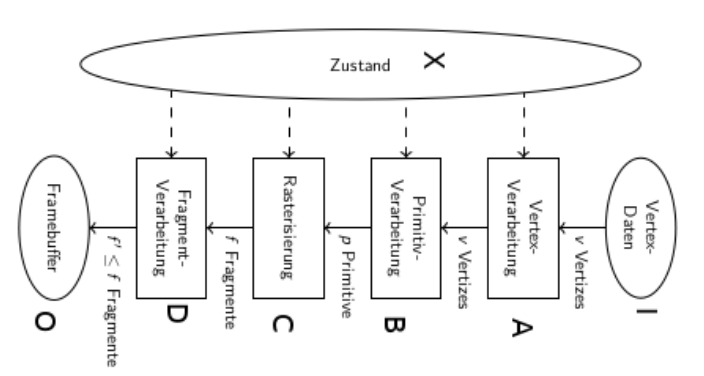
\includegraphics[scale=0.8]{1.png}

\indent \textbf{a)} Schema类型: (7p)

\begin{center}
    \begin{tabular}{|c|c|l|}
        \hline
        Stufe阶段&Benennung名称&Aufgabe任务\qquad\qquad\qquad\qquad\qquad\qquad\qquad\qquad\\
        \hline
        A&\textcolor{red}{Vertex顶点}&\dots\\
        \hline
        B&\textcolor{red}{Primitiv原始}&\\
        \hline
        C&\textcolor{red}{Rasterisierung栅格化}&\\
        \hline
        D&\textcolor{red}{Fragment分段}&\\
        \hline
        I&\textcolor{red}{Vertex-Daten}&\\
        \hline
        O&\textcolor{red}{Framebuffer帧缓冲区}&\\
        \hline
        X&\textcolor{red}{Zustand}&\\
        \hline
    \end{tabular}
\end{center}

\indent \textbf{b)}Datenfluss beschreiben bei n Dreiecken. 描述n个三角形的数据流。

\indent \textbf{c)}Welche 3 Shadertypen gibt es, die auf modernen GPUs programmierbar sind? 在现代GPU上可以编程哪三种着色器类型?

\indent \textbf{d)}Welche Stufe aus \textbf{a)} hat keinen programmierbaren Shader \& warum? (Rasterisierer: Coverage Tests gibt nur an ob Pixel innerhalb des Primitives ist.)
\textbf {a)}中的哪个级别没有可编程着色器\&为什么? (光栅器:覆盖率测试仅指示像素是否在图元内。)

\indent \textbf{e)}Single Buffering Speicher berechnen: 100x100Pixel 32Bit Color, 16Bit Depth wie viel Speicher wird benötigt? ( 100$\times$100$\times$ (32+16) Bit)
计算单个缓冲内存:100x100像素32位彩色,16位深度需要多少内存?

\indent \textbf{f)}Probleme von Single-Buffering? Wie viel Speicher wird zusätzlich benötigt? (Double-Buffering, VSync verwenden)
单缓冲有问题吗? 需要多少额外的内存? (使用双缓冲,VSync)

zu \textbf{b)} veranschaulicht插图: (videolink: \href{https://youtu.be/0PTBOX1HHIo?t=175}{Understanding the Graphics Pipeline}  )

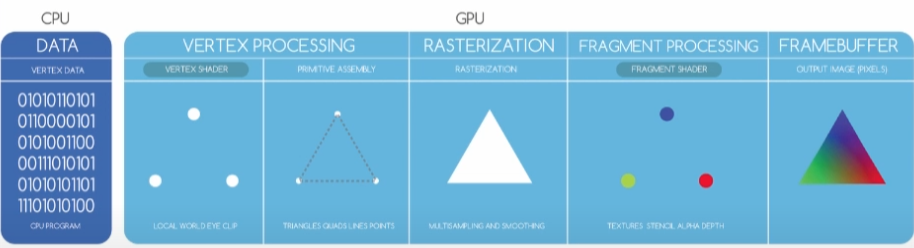
\includegraphics[scale=0.4]{2.png}
\\
\\
\textbf{2. Koordinaten-Transformation 坐标转换}

\indent\textbf{a)}Benennen sie die gängigsten Namen für die Matrizen M V P A. Welche Räume gibt es bei dem Ablauf der Pipeline? (Modell, View, Projektion, Viewport )
命名矩阵M V P A的最常用名称。管道中有哪些空间? (模型,视图,投影,视口)

\begin{center}
    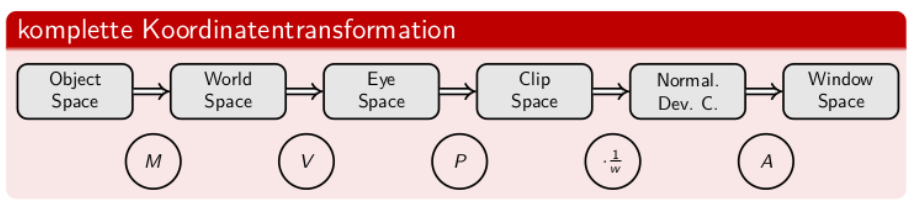
\includegraphics[scale=0.4]{3.png}
    
\includegraphics[scale=0.6]{4.png}
    \href{https://www-user.tu-chemnitz.de/~malo/CG-I}{WebGL-Anwendung zur Visualisierung der Koordinatentransformation}
\end{center}

\indent\textbf{b)}Welche Matrix verändert das Ergebnis/Wert (bspw. eines Tests) bzw. was sind die Eigenschaften der jeweiligen Matrizen?哪个矩阵会更改结果/值(例如测试),或者各个矩阵的属性是什么? 
\\(Tabelle mit unterschiedlichen Aufgaben dazu M V P A ankreuzen. 勾选将任务与M V P A分开的表) 
\\(Beispiel: welche Matrix hat Einfluss auf das Ergebnis des Tiefentests? 示例:哪个矩阵会影响深度测试的结果)

\indent\textbf{c)}Bild gegeben mit 4 Ansichten eines Schneemanns, der mit 5 Kugeln gezeichnet wurde. Wie viele unterschiedliche Matrizen braucht man? Begründe... (einzigstes  ,,Primitiv'' war die Kugel )

给定的图象有一个雪人的4个看法画与5个球。 您需要多少种不同的矩阵? 证明……(唯一的“原始”是球体)

Top \qquad | Left\qquad |   \qquad$\Rightarrow$ 4 Modell, 4 View, 2 Projektion, (Viewport bin ich mir nicht sicher, 

\hdashrule[0.5ex]{2.8cm}{1pt}{2mm} \,|\qquad\qquad\qquad\qquad\qquad\qquad\qquad\qquad\qquad denke aber 4 wegen Unterteilung)
    
Front \,\,\quad | Free

\noindent\textbf{3. Affine Abbildungen 仿射图像}

\indent\textbf{a)}Bild einer Transformation ähnlich wie aus der PVL dazu. Welche Matrizen wurden verwendet und wie sind die hintereinander gereiht worden?[Wie berechnet man die Modellmatrix? Reihenfolge!]
类似于PVL的转换图像。 使用了哪些矩阵,它们又是如何排列的[您如何计算模型矩阵? 顺序!]

\indent\textbf{b)} Punkt $P'$ ist gegeben. Berechnen sie $P$. ( $P' \times M^{-1}$ )
\\
\\
\noindent\textbf{4. Texturierung 纹理化}

\indent\textbf{a)} Vertices von Texturen rausfinden sehr ähnlich zur PVL. 找出纹理的顶点与PVL非常相似

\indent\textbf{b)} baryzentrische Koordinaten für Punkte berechnen. 计算点的重心坐标

\indent\textbf{c)} bilineare Filter erklären. 解释双线性滤波器

\noindent\textbf{5. Beleuchtung 灯光}

\indent\textbf{a)}Skizzen ergänzen. Unterschied zwischen Phong und Phong-Blinn. 完成草图。 Phong和Phong-Blinn之间的区别。 

\qquad $\Rightarrow$ Phong verwendet R, Phong-Blinn verwendet Winkelhalbierende H. Phong使用R,Phong-Blinn使用等分线H。

\indent\textbf{b)} Welches der beiden Algos ist effizienter? Phong-Blinn, da R schwieriger auszurechnen ist. 两种算法中哪一种效率更高? Phong-Blinn,因为R较难计算。

\indent\textbf{c)} Formel des Phong-Blinn Modells. Phong-Blinn模型的公式。

\indent\textbf{d)} Kann man mit Phong-Blinn Schatten erzeugen? 可以用Phong-Blinn制作阴影吗? $\Rightarrow$ (\href{https://youtu.be/lH61rdpJ5v8?t=461 }{OpenGL - lighting with the Phong reflection model (part 1 of 2)})

\noindent\textbf{6. Shading 底纹}

\indent\textbf{a)} Wofür braucht man das? Was ist das?

\indent\textbf{b)} Gourand, Phong Tabelle wo wirds beleuchtet? ( Mehrfachbennung möglich?) Gouraud,Phong桌子在哪里发光? (可能有多个答案?)

\begin{center}
    \begin{tabular}{|c|c|c|c|c|}
        \hline
        Shader &Pro Vertex&Pro Fragment& Vorteil\qquad\qquad\qquad\qquad&Nachteil\qquad\qquad\qquad\qquad\\
        \hline
        Gourand&&&&\\
        \hline
        Phong&&&&\\
        \hline
    \end{tabular}
\end{center}

\indent\textbf{c)} Welche notwendigen Daten müssen berechnet werden, bevor Phong-Blinn an Fragmenten ausgeführt werden kann? 在对碎片执行Phong-Blinn之前,必须计算哪些必要的数据?
\\
\\
\noindent\textbf{7. Rasterisierung 栅格化}

2 Dreiecke mit gemeinsamer Kante. Wie sorgt man dafür, dass es keine Löcher / Überschneidungen etc gibt. Wie erkennt man ob ein Pixel sich im Dreieck befindet? Warum funktioniert das?
2个具有共同边的三角形。 如何确保没有孔/重叠等。您如何知道像素是否位于三角形中? 为什么有效?

Wie wird versichert, dass keine doppelten Fragmente oder Löcher entstehen? 如何确保没有重复的碎片或孔?

Wieso ists wichtig, dass das lokal pro Dreieck entschieden wird? 为什么在每个三角形上局部确定该值很重要?

(Stichwort: Coverage Sample 覆盖样本)
\\
\\
\noindent\textbf{8. Clipping 剪裁}

Cohen-Sutherland 科恩·萨瑟兰

Code von Abstimmungen 投票守则

erkläre wofür jedes Bit steht 解释每一位代表什么

Punkte eintragen die während der Ausführung entstehen (+ den Code) 输入在执行过程中出现的点(+代码)

\begin{center}
    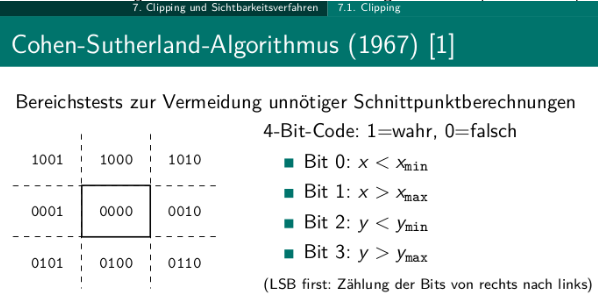
\includegraphics[scale=0.6]{5.png}
\end{center}

\noindent\textbf{9. Tiefenspeicher 深度存储 (Zusatz) +3}

8 Mbyte großer Framebuffer 4 MByte wird fürn Colorbuffer verwendet. 8 MB大帧缓冲区4 MB用于颜色缓冲区 

wie viele Objekte der Größe mit je 100 Fragmenten lassen sich erzeugen? (denke die Frage bezog sich aufn Tiefenbuffer) 可以创建多少个大小为100个碎片的对象? (认为​​问题与深度缓冲区有关)

\section{Klausur WS14/15}

\noindent\textbf{1. framework Pipeline 框架管道 (8p)}

Pipelinestufen 管道阶段:

- fragment Pipeline 片段管道,

- Vertex Pipeline 顶点管线,

- Primitive Pipeline 原始管道
\\
\\
\indent\textbf{a)} Ordnen Sie die die Arbeitsschritte den einzelnen Pipelinestufen zu: 6 Punkte
将工作步骤分配给各个管道阶段

- zTest/Tiefentest

- Transformation Eyespace -> ClipSpace

- BackfaceCulling 背面剔除

- Beleuchtung/Shading 照明/遮光

- Transformation Clipspace -> NormalizedDeviceSpace (?) 转换剪辑空间->规范化的设备空间

- Blending (?) 调和
\\
\\
\indent\textbf{b)} Begründen Sie die Einordnung der Beleuchtung/Shading. (vermutlich weil je nach Shading mode entweder vertices oder Fragmente Belekuchtet werden) (2 Punkte) 证明照明/阴影的分类合理。 (大概是因为根据阴影模式,顶点或片段会被照亮)
\\
\noindent\textbf{2. Affine Transformationen 仿射变换 (25 Punkte)}

\indent\textbf{a)} 3d-Punkt mit vorgegebenen Werten in homogene koordinaten "wandeln". (Punkt so was wie: (2,1,1) oder so)
将具有给定值的3D点"转换"为均匀坐标。 (点类似:(2,1,1)左右)

\indent\textbf{b)} Eine Matrix erstellen für Skalierung $x = 1/2, y = 1, z = 3/2$ und Rotation um Y-Achse um 450°.
创建一个矩阵来缩放$ x = 1/2,y = 1,z = 3/2 $并绕Y轴旋转450°。

\indent\textbf{c)} ViewMatrix gegeben: $\begin{pmatrix}
    1&0&0&4\\
    0&1&0&-2\\
    0&0&1&-1\\
    0&0&0&1
\end{pmatrix}$. 

Geben Sie die Kameraposition an. 指定相机位置。
(eine translation der Szene in die eine richtung entspricht der Bewegung der Kamera in die andere richtung entspricht. 场景在一个方向上的平移对应于相机在另一个方向上的移动。) 
\\
\\
\indent\textbf{d)} projektionsmatrix投影矩阵 gegeben: $\begin{pmatrix}
    1/2&0&0&0\\
    0&1/2&0&0\\
    0&0&5/3&8/3\\
    0&0&-1&0
\end{pmatrix}$

Ist dies eine perspektivische oder eine orthogonale Projektion? 这是透视图还是正交投影?
\\
\\
\indent\textbf{e)} gegeben: Modelmatrix模型矩阵 (vermutlich Lösung für \textbf{2b)})

Berechenen Sie für den Punkt aus Aufgabe \textbf{a)} die EyeSpace, ClipSpace und NormalizedDeviceSpace Position.
从例子\textbf {a)}计算该点的EyeSpace,ClipSpace和NormalizedDeviceSpace位置。

\indent\textbf{f)} Liegt der errechnete Punkt im Sichtbereich? Begründen Sie ihre Antwort. 计算的点在视野内吗? 解释你的回答。

\noindent\textbf{3. Blending调和 (10 Punkte)}

\indent\textbf{a)} Was ist Blending, wie geht lineares Blending? (6 Punkte) 什么是混合,线性混合如何工作?

\indent\textbf{b)} Zwei Bilder gegeben mit Hintergrundfarbe, Dreieck1 und Dreieck2. Farbwerte zu Hintergrund und Dreiecken gegeben (Ein Dreieck Alpha 0.5, das andere Alpha = 1.0).
给定具有背景色的两个图像,三角形1和三角形2.为背景和三角形给出的颜色值(一个三角形alpha 0.5,另一个alpha = 1.0)。

Es wurde etwas am rendervorgang gedreht, aber nciht an den Farben. Einmal wurden die Dreiecke im Überschneidungsbereich farblich gemischt, einmal nicht.  warum? (Tiefensortierung?!?)
在渲染过程中有一些旋转,但颜色没有旋转。 一旦重叠区域中的三角形混合了颜色,就一次不混合。 为什么? (深度排序?!?)
\\
\\
\noindent\textbf{4. AntiAliasing抗锯齿 (2 Punkte)}

Was bedeutet AntiAliasing?

\noindent\textbf{5. Beleuchtung 15 Punkte}

[Phong Beleuchtungsgleichnug gegeben; Spekularen und Diffusen Anteil vertauscht 给予Phong照明平等; 高光和散光零件已互换] Etwa:

k1 * i1 + \qquad\qquad\qquad\quad Anteil 1

k2 * i2 * u * <N,H>$^s$ + \, Anteil 2

k3 * i3 * <N,L> \qquad\qquad Anteil 3

\indent\textbf{a)} Benennen Sie die Anteile und beschreiben Sie, wie Sie das Aussehen beeinflussen. 命名零件并描述它们如何影响外观。

\indent\textbf{b)} ?

\indent\textbf{c)} Was ist H? Wie setzt es sich zusammen? 什么是H? 它是如何构成的?

\indent\textbf{d)} Was ist s? was beeinflusst es? 是什么s? 有什么影响?

\indent\textbf{e)} Zwei Bilder, beleuchtete Kugel; anscheinend einmal mit GouradShading (Vertices stechen hervor beim Glanzfleck) und einmal nach phong. 两个图像,照明的球体; 显然,一次使用GouradShading(顶点在光亮点突出),一次在phong之后。

Warum sieht das eine ,,schlechter'' aus wie das andere. Warum? Was muss man ändern, damit das schlechtere Bild besser aussieht. 为什么一个看起来比另一个更“差”。 为什么? 您必须更改什么才能使较差的画面看起来更好?

\section{Klausur WS12/13}

\noindent\textbf{1. Allgemeine Pipeline}

\begin{center}
    
\includegraphics[scale=0.6]{6.png}
\end{center}

\indent\textbf{a)} Ordnen sie die Begriffe den Pipelinestufen zu. 将定义分配给管道阶段 

\indent\indent A: ,,Attributinterpolation'' 属性插值

\indent\indent B: ,,Bresenham Algorithmus'' Bresenham算法

\indent\indent C: ,,Koordinatentransformation''

\indent\indent D: ,,Texturierung'' 纹理化
\\
\\
\indent\textbf{b)} Es wird meistens so gehandhabt, das der Rasterisierer (?) nur auf einem einzigen Vertices arbeitet, ohne informationen über das gesamte Polygon (oder sogar das Objekt) zu haben. Nennen sie ein Vorteil und ein Nachteil für dieses Vorgehen!通常以这样的方式进行处理:光栅化器(?)仅在单个顶点上起作用,而没有有关整个多边形(甚至对象)的信息。 列举这种方法的优点和缺点!

\indent\textbf{c)} ?

\indent\textbf{d)} Eine Kugel soll mit Dreiecken gerendert werden, nennen sie 2 Vorteile und Nachteile für dieses Vorgehen. 球形应使用三角形表示,此方法的名称和优点分别为2。
\\
\\
\noindent\textbf{2. Rasterisierung 栅格化}

\indent\textbf{a)} Was ist die grundsätzliche Idee des Bresenham Algorithmus zur Beschleunigung der Rastarisierung? [2 Pkt] Zusatz: Warum kann bei modernen Grafikprozessoren der naive Ansatz über die Geradengleichung dennoch besser sein? [1 Pkt]
Bresenham算法加速rastarization的基本思想是什么?另外:为什么在现代图形处理器中使用直线方程的幼稚方法会更好?

\indent\textbf{b)} Der Brasenham Algorithmus kann nur in mit Positiven Anstiegen arbeiten. Was muss man beachten wenn man ihn in alle Richtungen verwenden möchte?
Brasenham算法仅适用于正斜率。 如果要全方位使用它,应该考虑什么?

\indent\textbf{c)} Beschreiben sie kurz wie man den Bresenham Algorithmus verwenden könnte, wenn man ein Dreieck ausgefüllt rasterisieren möchte (also nicht nur die Linien)?
简要描述一下,如果要光栅化填充的三角形(不仅是直线),如何使用Bresenham算法?
\\
\\
\noindent\textbf{3. Antialiasing}

\indent\textbf{a)} Was versteht man Grundsätzlich unter ,,Aliasing''? “混叠”基本理解什么?

\indent\textbf{b)} Wie funktioniert Supersampling und wie wirkt es sich aus. Erläutere 2 Methoden. 超级采样是如何工作的,效果如何。 说明2种方法。

\indent\textbf{c)} Erläutere kurz das Multisampling als Spezialfall des Supersamplings. 简要说明多重采样是超级采样的特例。

\noindent\textbf{4. Affine Räume}

$a=\begin{pmatrix}
    1\\0\\2
\end{pmatrix},\,b=\begin{pmatrix}
    1\\2\\4
\end{pmatrix},\,c=\begin{pmatrix}
    1\\0\\-1
\end{pmatrix}$. Die Vektoren waren irgend wie so ähnlich.

\indent\textbf{a)} Nennen sie 4 Wichtige Affine Abbildungen! 提出4个重要的仿射图!

\indent\textbf{b)} Geben sie die Darstellung des Vektors a in homogenen Koordinaten an ( einfach 4. Komponente eine 1 hinzufügen)
给出向量在均质坐标中的表示(只需在第4个分量上加上1)

\indent\textbf{c)} Berechnen sie aus den \underline{homogenen} a, b und c die Normale in \underline{homogenen Koordinaten} für die Fläche.
根据\underline{均匀} a,b和c计算表面的\underline{均匀坐标}的法线。

\indent\textbf{d)} Es soll zuerst eine Translation T um (1,0,5) und danach eine Rotation R um die X-Achse um 90$^\circ$ durchgeführt werden. Geben sie T und R an.
首先应进行平移T乘(1,0,5),然后进行绕X轴的旋转R 90$^\circ$。 输入T和R。

\indent\textbf{e)} Berechnen sie eine Matrix M, welche die beiden Transformationen aus Aufgabe D vereint.
计算矩阵M,该矩阵M结合了练习D中的两个变换。

\indent\textbf{f)} Welche Transformation muss zur korrekten Darstellung der Normalen ausgeführt werden. Geben sie die Herleitung ohne genauen Werte an. [$N=(M^{-1})^T$]
为了正确表示法线,必须执行哪种变换。 给出没有精确值的推导。

\textbf{Zusatz:} Führen sie die Normalentransformation durch. 标准化
\\
\\
\noindent\textbf{5. Sichtbarkeitsverfahren 可见性/能见度程序 [12 Pkt]}

Gegeben sind die Verfahren \textbf{Z-Buffer Verfahren, Backface Culling, BSP-Baum Verfahren, Active Edge Table.} Beschreiben sie 3 der 4 Verfahren und gehen sie dabei auf die Notwendigen Datenstrukturen ein. 
描述4个过程中的3个,并说明必要的数据结构。

\textbf{Zusatz:} Erläutern Sie das verbleibende der 4 Verfahren! 解释其余4个步骤! [3 Pkt]
\\
\\
\noindent\textbf{6. Transformationen}

\begin{center}
    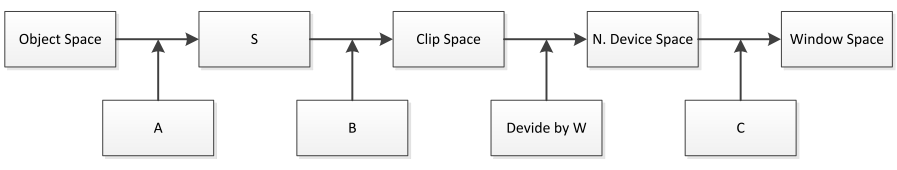
\includegraphics[scale=0.5]{7.png}
\end{center}

\indent\textbf{a)} Benennen sie die Teile A, B und C!

\indent\textbf{b)} Benennen sie S!

\indent\textbf{c)} (...) noch mehr...

\indent\textbf{d)} Bestimmen sie, ob es sich bei der gegebenen Matrix um eine Ortogonale oder Perspektivische Transformation handelt. Begründen sie!
确定给定的矩阵是正交变换还是透视变换。 说明!

$$\begin{pmatrix}
    1/2&1/4&0&a\\
    -1/8&5/2&0&b\\
    0&0&1&2\\
    0&0&1/(-d)&0
\end{pmatrix}$$

\indent\textbf{e)} Ein Quadrat wird mit der Matrix Projiziert, welches Seitenverhältnis hat es hinterher? 
用矩阵投影一个正方形,之后它具有什么纵横比?

\indent\indent Begründen Sie ihre Antwort!

\noindent\textbf{7. Farbmodelle 颜色模型}

\begin{center}
    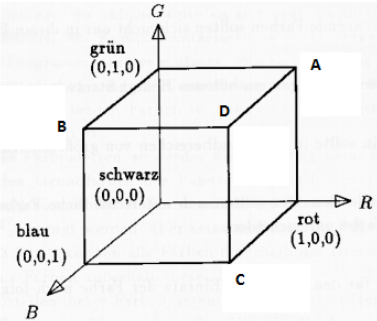
\includegraphics[scale=0.6]{8.png}
\end{center}

\indent\textbf{a)} Benennen Sie die fehlenden Farben A, B, C und D korrekt!
正确提出缺少的颜色A,B,C和D!

\indent\textbf{b)} Welches der anderen Farbmodelle ist bei dem vorliegendem RGB Modell sofort ersichtlich? 
在当前的RGB模型中,哪个其他颜色模型立即可见?

\indent\indent Geben sie die Umrechnungsformel für die beiden Farbmodelle an!
输入两种颜色模型的转换公式!

\indent\textbf{c)} Begründen sie welches der beiden Farbmodelle ein additives und welches ein subtraktives Farbmodell ist! 
证明两个颜色模型中的哪个是加色模型,哪个是减色模型!

\indent\indent Ordnen Sie beiden Verfahren eine Anwendung zu. 为这两个过程分配一个应用程序。
\\
\\
\noindent\textbf{8. Beleuchtung 灯光}
\begin{center}
    \begin{equation}
        \begin{aligned}
            I=& k_1\cdot I_1 + & Anteil 1\\
            & k_2\cdot I_2\cdot <N,L>+ & Anteil 2\\
            & k_3\cdot I_3\cdot u \cdot <N,H>^s & Anteil 3
        \end{aligned}
    \end{equation}
\end{center}

\indent\textbf{a)} Benennen Sie die Anteile! 说明各个部分。

\indent\textbf{b)} Was beschreibt der 1. Anteil und warum sollte der Wert nicht zu hoch gewählt werden?
第一部分描述什么,为什么值不应该过高?

\indent\textbf{c)} Was besagt das Lambertsche Gesetz? \textbf{Zusatz:} Was wäre, wenn u dauerhaft den Wert 1 hätte?
兰伯特定律怎么说?如果u永久拥有值1怎么办?

\indent\textbf{d)} Was ist der H Vektor im 3. Anteil und wie berechnet man ihn? Verdeutlichen sie die Vektoren mit einer Skizze.
第三部分的H向量是什么,如何计算? 用草图使向量清晰。

\indent\textbf{e)} Es wird meistens nur Lokale Beleuchtung Modelliert. Nennen sie ein Vorteil und ein Nachteil davon. 
通常仅模拟本地照明。 给它们命名一个优点和缺点。

\indent\indent\textbf{Zusatz:} Nennen Sie ein globales Beleuchtungsverfahren!
提出全局照明方法!

\indent\textbf{f)} Was ist der Unterschied zwischen Flat Shading, Gouraud Shading und Phong Shading? Ordnen sie die Begriffe ,,Per Pixel Lightning'' und ,,Per Vertex Lightning'' korrekt zu!

Flat Shading,Gouraud Shading和Phong Shading有什么区别? 正确分配术语“每像素闪电”和“每顶点闪电”!
\\
\\
\noindent\textbf{9. }

\indent\textbf{a)} Was versteht man ganz Allgemein unter ,,Texturieren''? 一般而言,“纹理化”是什么意思?

\indent\textbf{b)} Was ist der Unterschied zwischen prozeduralen und diskreten Texturen? 程序纹理和离散纹理之间有什么区别?

\newpage

\section{PVL 1 - Rasterbilder, Displayschnittstellen, Mathematische Grundlagen}

\noindent\textbf{1. Rasterbilder 光栅图像}

Zur Repräsentation von Rasterbilddaten wird meist ein zweidimensionales Array von Pixeldaten verwendet. Wir betrachten den Fall, dass pro Pixel ein Rot-, Grün-, Blau- sowie Alpha-Anteil gespeichert werden soll\footnote{Der Alpha-Kanal selbst trägt dabei nicht direkt zur Farbe bei, sondern erlaubt das Speichern von Zusatzinformationen, wie zum Beispiel Transparenz. Alpha通道本身并不直接对颜色有贡献,但是允许保存其他信息,例如 透明度。}. Pro Kanal werden überlicherweise 8 Bit verwendet, so dass die Intensität jedes Anteils in 256 Stufen kodiert werden kann.

像素数据的二维阵列主要用于表示光栅图像数据。 我们考虑了为每个像素存储红色,绿色,蓝色和Alpha分量的情况。 通常每个通道使用8位,因此每个分量的强度可以编码为256级。

Der Hauptspeicher eines Rechners kann als eine Folge von jeweils 1 Byte großen Speicherzellen aufgefasst werden, die über eine eindimensionale Addresse referenziert werden. Zur Speicherung eines Rasterbildes werden die einzlenen Pixel zeilenweise nacheinander im Speicher abgelegt.

可以将计算机的主存储器理解为通过一维地址引用的一系列1字节大存储单元。 为了存储光栅图像,将各个像素一个接一个地存储在存储器中。

\begin{center}
    
\includegraphics[scale=0.4]{9.png}
\end{center}

\indent\textbf{(a)} Berechnen Sie den Speicherbedarf für ein Bild der Auflösung 4096 $\times$ 2160 Pixel (,,4K2K'') im oben beschriebenem RGBA-Format! (1 Punkt) 求上述RGBA格式计算分辨率为4096$\times$2160像素("4K2K")的图像的内存需求!

\indent\textbf{(b)} Wir betrachten ein Bild mit Auflösung $w\times h$. Geben Sie eine Formel $a(x, y, c)$ an, die für eine gegebene zweidimensionale Pixelposition $(x, y)$ mit $x\in \{0, . . . , w − 1\}, y \in \{0, . . . , h − 1\} $ sowie dem KanalIndex $c \in \{0, 1, 2, 3\}$ (0 für rot, 1 für grün, usw.) die Speicheradresse bestimmt! (Das Bild beginne bei Adresse 0). (1 Punkt)

\indent\textbf{(c)} Geben Sie Formeln oder einen Algorithmus an, mit dem aus einer gegebenen Adresse $m$ (und in Abhängigkeit von den Parametern Bildbreite $w$ sowie Bildhöhe $h$) die zweidimensionale Pixelposition $(x, y)$ sowie der Kanal-Index $c$ rekonstruiert werden kann. Ihre Funktion / Ihr Algorithmus soll dazu auf die Parameter $w$ und $h$ zurückgreifen. Bestimmen Sie dann die Pixelposition sowie den Kanal-Index, der an Adresse $m = 4189$ eines 77 $\times$ 50 Pixel großen Bildes gespeichert wird. (3 Punkte)
给出公式或算法,利用该公式或算法可以从给定的addressem(并取决于图像宽度和图像高度h)重建二维像素位置(x,y)和通道索引。 为此,您的函数/算法应使用参数w和h。 然后确定像素位置和通道索引,将其存储在77x50像素图像的Adressem = 4189处。

\indent\textbf{(d)} Berechnen Sie $w$ und $h$, wenn das Bild insgesamt 92160 Byte groß ist, und das Pixel (42, 23) an der Adresse 14888 beginnt! (2 Punkte)
如果图像总计92160字节并且像素(42.23)从地址14888开始,请计算w和h!
\\
\\
\noindent\textbf{2. Displayschnittstellen 显示界面}

Ein LCD-Monitor mit der Auflösung 2560 $\times$ 1440 Pixel wird mit einem digitalen 60Hz Videosignal versorgt (unkomprimiert, RGB, 8Bit pro Kanal)

分辨率为2560$\times$1440像素的LCD监视器配有60Hz数字视频信号(未压缩,RGB,每通道8位)

\indent\textbf{(a)} Welche Datenrate (in MB/s, gerundet auf 1 Stelle nach dem Komma, Si-Notation ein Megabyte=$10^6$ Byte) muss die Displayschnittstelle mindestens zur Verfügung stellen? (1 Punkt)
显示界面必须提供的最低数据速率是多少?

\indent\textbf{(b)} Das Videosignal wird mit einer DVI-D-Schnittstelle übertragen. Dabei ergibt sich ein Pixeltakt von 241,7 MHz statt der naiv zu erwartenden 221,2 MHz. Erklären Sie, wodurch der höhere Pixeltakt zu Stande kommt! (2 Punkte)
视频信号通过DVI-D接口传输。 这导致241.7 MHz的像素时钟,而不是天真预期的221.2 MHz。 说明更高的像素时钟是如何产生的!
\\
\\
\noindent\textbf{3. Mathematische Grundlagen}



Gegeben seien die Punkte:

$A=\begin{pmatrix}
    0\\0\\2
\end{pmatrix},\,B=\begin{pmatrix}
    4\\0\\2
\end{pmatrix},\,C=\begin{pmatrix}
    -2\\2\\0
\end{pmatrix},\,P=\begin{pmatrix}
    2\\3\\3
\end{pmatrix},\,Q=\begin{pmatrix}
    2\\5\\5
\end{pmatrix}$
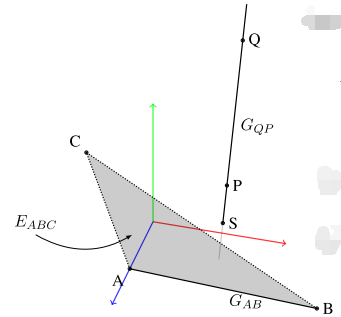
\includegraphics[scale=0.5]{10.png}

\indent\textbf{(a)} Bestimmen Sie die Geradengleichung für die Geraden $G_{QP}$ und $G_{AB}$ in expliziter Form.
以显式形式确定直线$G_{QP}$和$G_{AB}$的直线方程。

\indent\textbf{(b)} Die drei Punkte $A,B$ und $C$ spannen eine Ebene auf. Bestimmen Sie die Ebenengleichung der Ebene $E_{ABC}$ in impliziter, sowie expliziter Form. (2p)
A,B和C这三个点跨越一个平面。 确定隐式和显式形式的EABC平面的平面方程。

\indent\textbf{(c)} Berechnen Sie den euklidischen Abstand zwischen folgenden Objekten:
计算以下对象之间的欧几里得距离:

\indent\indent- der Geraden $G_{AB}$ und $G_{QP}$ 

\indent\indent- der Ebene $E_{ABC}$ und dem Punkt $Q$ 

\indent\indent- der Ebene $E_{ABC}$ und der Geraden $G_{QP}$ 

\indent\indent- der \textbf{Strecke} $PQ$ und dem Punkt $C$

\indent\textbf{(d)} Berechnen Sie den Schnittpunk S zwischen der Geraden $G_{PQ}$ und der Ebene $E_{ABC}$.
\\
\\
\noindent\textbf{PVL 1 - Antwort}

\indent\textbf{1. Rasterbilder}

\indent\indent\textbf{(a)} $4\cdot 4096\cdot 2160 = 35389440$ Bit

\indent\indent\textbf{(b)} $a\cdot (x,y,c) = y\cdot w\cdot 4+x\cdot 4+(c+1)-1=(y\cdot w+4)\cdot 4 + c$

\indent\indent\textbf{(c)}
\begin{lstlisting}
    def func(m): 
        y = (m + 1) / (4*w) 
        h = (m + 1) % (4*w) / 4 
        c = m % 4 
        return (x,y,c)
    y = 13 
    x = 46 
    c = 1
\end{lstlisting}

\indent\indent\textbf{(d)}

\indent\indent\indent14888\% 4 = 0 $\Rightarrow c=0$

\indent\indent\indent$(42+23\cdot w)\cdot 4 +c=14888$

\indent\indent\indent$4\cdot w\cdot h=92160\Rightarrow w=160,\,h=144$

\indent\textbf{2. Displayschnittstellen}

\indent\indent\textbf{(a)} $2560\cdot 1440\cdot 3\cdot 8\cdot 60\cdot 125/10^9 \approx 663.3552\, MB/s$

\indent\indent\textbf{(b)} Der Pixeltakt zeigt, dass die Menge der Pixel, die an den Monitor pro Sekunde gesendet werden. Die inaktiven Pixel werden auch gezählt. Es wird vom produkt der totalen horizontalen Pixelzahl und der Zeilenfrequenz errechnet.
像素时钟显示每秒发送到显示器的像素数量。 不活动像素也被计数。 它是根据水平像素总数与行频的乘积计算得出的。
$$f_{P_x}=Spaltenanzahl \times Bildwiederholfrequenz \times (Zeilenanzahl + Austastzeilen)$$

\indent\textbf{3. Mathematische Grundlagen}

\indent\indent\textbf{(a)} 
$$G_{QP} :=\frac{x-2}{2-2}=\frac{y-3}{5-3}=\frac{z-3}{5-3}\Rightarrow x=2,\,y=z$$
$$G_{AB} :=\frac{x-0}{4-0}=\frac{y-0}{0-0}=\frac{z-2}{2-2}\Rightarrow x=0,\,y=2$$

\indent\indent\textbf{(b)}
$$\overrightarrow{AB}=\begin{pmatrix}
    4\\0\\0
\end{pmatrix},\,\overrightarrow{AC}=\begin{pmatrix}
    -2\\2\\-2
\end{pmatrix},\,\vec{n}=\overrightarrow{AB}\times \overrightarrow{AC}=\begin{pmatrix}
    0\\8\\8
\end{pmatrix}$$
        
$$ d=-16,\,8y+8z-16=0\rightarrow\left\{
\begin{aligned}
    &y+z-2=0 & impliziter Form\\
    &y=2-z & expliziter Form
\end{aligned}
\right.
$$

\indent\indent\textbf{(c)}

Abstand zwischen $G_{AB}$ und $G_{QP}$ :

$$\vec{n}=\overrightarrow{AB}\times\overrightarrow{QP}=\begin{pmatrix}
    0\\8\\-8
\end{pmatrix}$$

$$d=\frac{|\overrightarrow{AQ}\cdot\vec{n}|}{|\vec{n}|}=\frac{\left|\begin{pmatrix}2\\5\\3\end{pmatrix}\cdot\begin{pmatrix}0\\8\\-8\end{pmatrix}\right|}{\left|\begin{pmatrix}0\\8\\-8\end{pmatrix}\right|}$$

\indent\indent\indent Abstand zwischen $E_{ABC}$ und $Q$:

$$E_{ABC}:\,y+z-2=0$$

$$d=\frac{|A_{x0}+B_{y0}+C_z+D|}{\sqrt{A^2+B^2+C^2}}=\frac{|0\cdot 2+5+5-2|}{\sqrt{0^2+1^2+1^2}}=4\sqrt{2}$$

\indent\indent\indent Abstand zwischen $E_{ABC}$ und $G_{QP}$: Weil $G_{QP}$ und $E_{ABC}$ schneidet, ist $d=0$

\indent\indent\indent Abstand zwischen \textit{Strecke} $PQ$ und $C$:
$$d=\sqrt{(2-(-2))^2+(3-2)^2+(3-0)^2}=\sqrt{26}$$

\indent\indent\textbf{(d)}

$$G_{PQ}:\left\{
    \begin{aligned}
       x=2\\y=z
    \end{aligned}
    \right.$$
$$E_{ABC}:y+z-2=0\Rightarrow x=2,\,y=2=1.\qquad S=\begin{pmatrix}
    2\\1\\1
\end{pmatrix}$$

\newpage

\section{PVL 2 - Bresenham für beliebigen Anstieg, Rasterisierungsqualität, Bresenham-Verfahren}

\noindent\textbf{1. Bresenham für beliebigen Anstieg 布雷森汉姆的任何倾斜}

Der klassische Bresenham-Algorithmus wie er in der Vorlesung vorgestellt wurde funktioniert
 nur für Linien mit Anstiegen im Bereich [0, 1], d.h. Linien die in x-Richtung schneller 
 ansteigen als in y-Richtung und die von links unten nach rechts oben gezeichnet werden. 
 Somit können nur Linien mit Anstiegen innerhalb des I. Oktanten gezeichnet werden, 
 wie nebenstehend abgebildet.
 讲座中介绍的经典Bresenham算法仅适用于斜率在[0,1]范围内的线,即 在x方向上比在y方向上上升更快的线是从左下到右上绘制的。 这意味着只能绘制第一个八分位数内增加的线,如右图所示。

Der Algorithmus lässt sich jedoch für Linien beliebiger Anstiege erweitern. 
Das folgende Pseudocode-Programmfragment zeigt den Bresenham-Algorithmus in 
verallgemeinerter Form (links) im Vergleich zu seiner einfachen Form (rechts). 
Als Eingabe erhält er die Koordinaten des Startpunktes $(x_0, y_0)$ und des Endpunktes $(x_1, y_1)$.
但是,该算法可以扩展到任何斜率的线。 以下伪代码程序片段以广义形式(左)与简单形式(右)相比显示了Bresenham算法。 作为输入,他接收起点(x0,y0)和终点(x1,y1)的坐标。

\begin{center}
    
\includegraphics[scale=0.6]{11.png}
    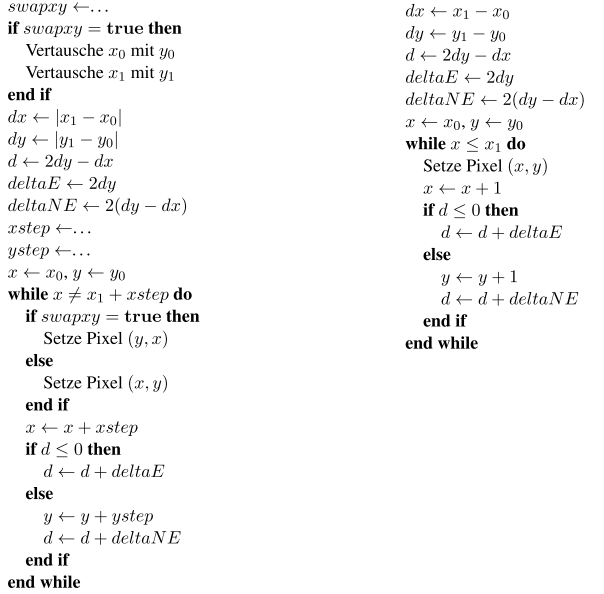
\includegraphics[scale=0.6]{12.png}
\end{center}

\indent\textbf{(a)} Geben Sie an, welche Werte die Variablen \textit{swapxy}, \textit{xstep} und \textit{ystep} für Linien mit Anstiegen in den abgebildeten Oktanten annehmen müssen! (7 Punkte)
指定显示的八进制数增加的行的变量swapxy,xstep和ystep必须具有哪些值!

\begin{center}
    \begin{tabular}{c|c|c|c|c|c|c|c|c}
        Variable &I&II&III&IV&V&VI&VII&VIII\\
        \hline
        \hline
        \textit{swapxy}&&&\textbf{true}&&&&&\\
        \hline
        \textit{xstep}&&&1&&&&&\\
        \hline
        \textit{ystep}&&&-1&&&&&
    \end{tabular}
\end{center}

\indent\textbf{(b)} Ergänzen Sie für die im obigen Algorithmus verwendeten Variablen \textit{swapxy}, \textit{xstep} und \textit{ystep} die entsprechenden Berechnungsvorschiften (gekennzeichnet durch . . . )! (3 Punkte)
为上述算法中使用的变量swapxy,xstep和ystep添加相应的计算规则
\\
\\
\noindent\textbf{2. Rasterisierungsqualität 栅格化质量}

Geben Sie für jeden der folgenden Fälle (\textit{a}) bis (\textit{e}) jeweils eine Begründing dafür an, wieso die dargestellte Linie nicht mit dem Bresenham-Algorithmus entstanden sein kann!
对于以下每种情况(a)至(e),说明为什么无法使用Bresenham算法创建所示行的原因!

\begin{center}
    
\includegraphics[scale=0.5]{13.png}
\end{center}

\noindent\textbf{3. Bresenham-Verfahren 布雷森汉法}

Wir betrachten den Bresenham-Algorithmus im I. Oktanden, wie er im Pseudocode zu Aufgabe 1 auf der rechten Seite gegeben ist. Bekannt sei lediglich der Ablauf der ersten fünf Iterationen der Schleife:
我们在右边的练习1的伪代码中给出了在第1个八度中的Bresenham算法。 只有循环的前五个迭代的序列是已知的:

\begin{center}
    \begin{tabular}{cc}
        1.Iteration & Setze Pixel (2,2)\\
        &$x\leftarrow 3$\\
        &$d\leftarrow 5$\\
        \hline
        2.Iteration & Setze Pixel (3,2)\\
        &$x\leftarrow 4$\\
        &$y\leftarrow 3$\\
        &$d\leftarrow -3$\\
        \hline
        3.Iteration & Setze Pixel (4,3)\\
        &$x\leftarrow 5$\\
        &$d\leftarrow 3$\\
        \hline
        4.Iteration & Setze Pixel (5,3)\\
        &$x\leftarrow 6$\\
        &$y\leftarrow 4$\\
        &$d\leftarrow -5$\\
        \hline
        5.Iteration & Setze Pixel (6,4)\\
        &$x\leftarrow 7$\\
        &$d\leftarrow 1$\\
    \end{tabular}
\end{center}

\indent Bestimmen Sie den Start- und Endpunkt der Linie! Geben Sie Ihren Lösungsweg an!
确定直线的起点和终点! 提供您的解决方案!
\\
\\
\noindent\textbf{PVL 2 - Antwort}

\indent\textbf{1.}

\indent\indent\textbf{(a)}

\begin{center}
    \begin{tabular}{c|c|c|c|c|c|c|c|c}
        Variable &I&II&III&IV&V&VI&VII&VIII\\
        \hline
        \hline
        \textit{swapxy}&false&true&\textbf{true}&false&false&true&true&false\\
        \hline
        \textit{xstep}&1&1&1&-1&-1&-1&-1&1\\
        \hline
        \textit{ystep}&1&1&-1&1&-1&-1&1&-1
    \end{tabular}
\end{center}

\indent\indent\textbf{(b)}

\begin{lstlisting}
    if dx < dy then swapxy <- true else swapxy <- false end if
    if x0 < x1 then xstep <- 1 else xstep <- -1 end if
    if y0 < y1 then ystep <- 1 else ystep <- -1 end if
\end{lstlisting}

\indent\textbf{2.}

\indent\indent\textbf{(a)} Bei jedesmal Schleife wird y um r akkumuliert, wenn es $r\in[0,1]$ keine Sprigen gibt.
在每个循环中,如果没有分支,则y由r累加。

\indent\indent\textbf{(b)} es ist unmöglich, wenn y3 == y2 und y3 == y2 + 1 ist.

\indent\indent\textbf{(c)} Aufgrund jedesmal 1 addierte x wird es jede Spalte 1 Pixel gegeben. Deswegen sollte in X-achse keine Zerbrechen. 
因为x每次都会添加,所以每列有1个像素。 因此,X轴不应断裂。

\indent\indent\textbf{(d)} ähnlich wie (b). Es ist nicht möglich, wenn y5 == y4 und y5 == y4 + 1 ist.

\indent\indent\textbf{(e)} Die Linie ist im Bresenham-Algorithmus immer steigend. D.h. gibt es keine sinkende Möglichkeit.
在Bresenham算法中,这条线一直在上升。 即 没有下沉的可能性。
\\
\\
\indent\textbf{3.}

$$d=d+\Delta E = 2dy-dx+2dy=4dy-dx=4\cdot(y_1-y_0)-(x_1-x_0)$$
$$\rightarrow4\cdot(y_1-2)-x_1-2=5$$

$$d=d+\Delta NE=d_{last}+2\cdot(dy-dx)=d_{last}+2\cdot(y_1-y_0)-2\cdot(x_1-x_0)=-3$$
$$\rightarrow 5+2\cdot(y_1-2)-2\cdot(x_1-2)=-3$$

$$\Rightarrow x_1=9,\,y_1=5$$

\newpage

\section{PVL 3 - Render-Pipeline, Lineare Interpolation, Lineare Interpolation im Dreieck}

\noindent\textbf{(a) Vorbemerkung: Indexed Rendering 初步评论:索引渲染}

In der CG1-Übung betrachten wir eine Renderpipeline, 
die als Eingabe ein Array von Vertizes erwartet, 
welches einzelne Primitive sequentiell kodiert. 
Sollen zum Beispiel drei Dreiecke verarbeitet werden, 
so benötigen wir ein Array von 9 Vertizes. 
In der Praxis ergeben sich häufig Situationen, 
in denen sich benachbarte Dreiecke eine gemeinsame Kante teilen, 
d.h. wir müssen absolut identische Vertizes mehrmals in das Vertex-Array aufnehmen – je einmal für jedes Primitiv, 
in dem sie gebraucht werden. 

在CG1练习中,我们考虑了一个渲染管线,该管线期望将一组顶点作为输入,并按顺序对各个图元进行编码。 例如,如果要处理三个三角形,则需要9个顶点的数组。 在实践中,经常出现相邻三角形共享公共边的情况。 我们必须在顶点数组中多次包含绝对相同的顶点,对于需要它们的每个图元一次。

GPUs und Render-APIs wie OpenGL unterstützen darüber hinaus das sogenannte \textit{Indexed Rendering}.
 Dabei spezifiziert das Vertex Array die Menge aller vorkommenden Vertizes, 
 aber die eigentlichen Primitive werden durch ein zusätzliches Array von \textit{Indizes} spezifiziert, welche jeweils einen bestimmten Vertex referenzieren. In der Abbildung sind die beiden Varianten gegenübergestellt:

GPU和渲染API(例如OpenGL)也支持所谓的索引渲染。 顶点数组指定所有出现的顶点的集合,但是实际图元由附加索引数组指定,每个索引都引用某个顶点。 下图中比较了两个变体:

\begin{center}
    
\includegraphics[scale=0.6]{14.png}
\end{center}

Im Beispiel benötigen wir also nur ein Vertex-Array mit 4 statt 9 Elementen, 
wenn mit Indexed Rendering gearbeitet werden kann, 
allerdings wird zusätzlich ein Index-Array mit 9 Einträgen benötigt. 

在此示例中,如果可以使用IndexedRendering,我们只需要一个包含4个元素(而不是9个元素)的顶点数组,但是,还需要具有9个条目的索引数组。

\noindent\textbf{Aufgabe} 

Es soll eine Pyramide mit quadratischer Grundfläche gerendert werden. Jeder Vertex werde durch die folgenden Attribute beschrieben:

将渲染具有正方形底的金字塔。 每个顶点由以下属性描述:

- Position (3D-Koordinaten), beschrieben als 3 $\times$ 32Bit Fließkommazahlen 浮点数字

- Farbe (RGB-Vektor), beschrieben als 3 $\times$ 32Bit Fließkommazahlen

Falls Indexed Rendering zum Einsatz kommt, so soll jeder Index durch einen 32Bit-Integerwert repräsentiert werden. Es sollen nun die folgenden vier Fälle betrachtet werden:

如果使用索引渲染,则每个索引应由32位整数值表示。 现在将考虑以下四种情况:

A: die gesamte Pyramide soll einfarbig blau dargestellt werden

B: die erste Seitenfläche soll rot, die zweite grün, die dritte gelb, die vierte violett und die Grundfläche weiß erscheinen (es soll aber nirgends ein Farbverlauf innerhalb einer Fläche entstehen)

C: die Spitze der Pyramide soll weiß sein, auf jeder der vier Seitenflächen soll ein Farbverlauf von weiß an der Spitze zu blau an der Unterkante entstehen, und die Grundfläche soll einfarbig blau sein

D: die Spitze der Pyramide soll weiß sein, auf jeder der vier Seitenflächen soll ein Farbverlauf von weiß an der Spitze zu blau an der Unterkante erscheinen, und die Grundfläche soll einfarbig grün sein

A:整个金字塔应以蓝色显示

B:第一个侧面应显示为红色,第二个绿色应显示为第三种黄色,第四个紫色应为紫色,而底面应为白色(但在任何区域内均不应出现颜色渐变)

C:金字塔的顶部应该是白色的,在四个侧面的每个侧面上,应该创建从顶部白色到底部边缘蓝色的颜色渐变,并且底部应该是纯蓝色

D:金字塔的顶部应为白色,四个侧面的每一个上均应出现从顶部白色到底部边缘蓝色的颜色渐变,并且底色应为纯绿色

Geben Sie jeweils die \textbf{minimale} Anzahl an Vertizes und Primitiven an, die nötig sind, um den Fall mit und ohne Indexed Rendering umzusetzen, sowie den sich dadurch ergebenden Speicherbedarf (Vertex Array + ggf. Index Array)! (Als Primitivtyp sollen immer Dreiecke verwendet werden.) (6 Punkte)

指定实现带或不带索引渲染的情况所需的最小顶点和图元数量,以及产生的内存要求(顶点数组+可能是索引数组)! (三角形应始终用作基本类型。)

\begin{center}
    \begin{tabular}{|c|c|c|c|c|}
        \hline
        Fall&Indexed Rendering&Anzahl Vertizes&Anzahl Primitive&Speicherbedarf(Bytes)\\
        \hline
        A&nein&&&\\
        \hline
        A&ja&&&\\
        \hline
        B&nein&&&\\
        \hline
        B&ja&&&\\
        \hline
        C&nein&&&\\
        \hline
        C&ja&&&\\
        \hline
        D&nein&&&\\
        \hline
        D&ja&&&\\
        \hline
    \end{tabular}
\end{center}

\noindent\textbf{(b)}

Wir betrachten einen Framebuffer in der Auflösung w $\times$ h Pixel. Es soll eine einzelne Linie gerendert werden, wobei ein Standard-Algorithmus zur Linienrasterisierung (Linienbreite ein Pixel, kein AntiAliasing) zum Einsatz komme, z.B. der Bresenham-Algorithmus. 

我们考虑分辨率为w$\times$h像素的帧缓冲区。 使用用于线光栅化的标准算法(线宽一个像素,无抗锯齿)来渲染单条线,例如 Bresenham算法。

Wie hoch ist die minimale und die maximale Anzahl an Fragmenten, die sich beim Rendern ergeben können, wenn Sie Start- und Endpunkt der Linie frei wählen können? Geben Sie für das Minimum und das Maximum jeweils ein Beispiel dafür an, wie Start- und Endpunkt und gewählt werden müssen, um den Fall zu erreichen! (Es genügt, ein Beispielszenario in Worten zu beschreiben, es müssen keine konkreten Koordinaten angegeben werden.) (2 Punkte)

如果您可以自由选择线的起点和终点,那么可以产生渲染的片段的最小和最大数量是多少? 对于最小值和最大值,请举一个示例,说明如何选择起点和终点才能达到目标! (用语言描述示例场景就足够了,不必给出特定的坐标。)
\\
\\
\noindent\textbf{(c)}

Es werden beginnend ab dem Zeitpunkt $t_0 = 0$ nacheinander 5 Frames einer Animation gerendert. 
 Die Renderzeit der Frames betrage $f_1 = 15ms, f_2 = 10ms, f_3 = 5ms, f_4 = 30ms$ und $f5 = 5ms$.
 Der angeschlossene Monitor arbeite mit eine Bildwiederholfrequenz von 50Hz. 
 Wir gehen vereinfachend davon aus, dass ein Vertical Blanking Interval\footnote{Ein \textit{Vertical Blanking Interval} (deutscher Fachbegriff: \textit{vertikale Austastlücke}) beschreibt die Zeit zwischen der Übertragung der letzen Zeile eines Frames und der Übertragung der ersten Zeile des Folgeframes. 垂直消隐间隔描述了帧的最后一行的传输与下一帧的第一行的传输之间的时间。} unendlich kurz ist, und auch ein \textit{Buffer Swap} keine Zeit verbraucht. Bekannt sei, dass ein Vertical Blanking Intervall zum Zeitpunkt $t_{vblank} = 10ms$ stattfindet. Es sollen drei Fälle betrachtet werden:

从时间t0 = 0开始,动画的5帧一个接一个地渲染。 帧的渲染时间为f1 = 15ms,f2 = 10ms,f3 = 5ms,f4 = 30ms和f5 = 5ms。 连接的显示器以50Hz的刷新率工作。 为简单起见,我们假定垂直消隐间隔无限短,并且缓冲区交换不会消耗任何时间。 已知在时间tvblank = 10ms发生垂直消隐间隔。 应考虑三种情况:

 A: Single-Buffering 单缓冲 (Rendern direkt in den \textbf{FRONT}-Buffer) 
 
 B: Double-Buffering ohne ,,VSync'' 
 
 C: Double-Buffering mit ,,VSync''

Berechnen Sie für die Fälle \textbf{A} bis \textbf{C}, zu welchem Zeitpunkt sich im \textbf{FRONT}-Buffer frühestens Bildteile (nicht notwendigerweise das finale Bild!) von Frame 5 befinden können! (3 Punkte)

对于情况A到C,计算帧5的图像部分(不一定是最终图像!)可以在FRONT缓冲区中的最早时间点!
\\
\\
\noindent\textbf{2. Lineare Interpolation 线性插值}

Gegeben sei eine Linie mit den Endpunkten $A=\begin{pmatrix}
    -3\\3
\end{pmatrix}$ und $B=\begin{pmatrix}
    6\\0
\end{pmatrix}$.
Den Punkten seien dabei die jeweiligen Farbwerte $c_A = (0, 0, 1)$ und $c_B = (1, 0, 1)$ zugeordnet. Die Farbwerte aller weiteren auf dieser Linie befindlichen Punkte ergeben sich damit als lineare Interpolation der Farbwerte der Endpunkte, sodass ein weicher Farbverlauf von \textbf{A} nach \textbf{B} entsteht

给定一条带有端点A和B的线。分别将颜色值cA =(0,0,1)和cB =(1,0,1)分配给这些点。 位于该线上的所有其他点的颜色值是端点颜色值的线性内插结果,因此创建了从A到B的柔和的颜色渐变

\indent\textbf{(a)} Nennen Sie eine allgemeine Formel zur Berechnung des Wertes $c$ als lineare Interpolation zwischen den Werten $a$ und $b$ in Abhängigkeit eines Parameters $t\in [0, 1]$, so dass bei $t = 0$ der Wert $a$ und bei $t = 1$ der Wert $b$ angenommen wird! (1 Punkt)
给出一个通用公式,用于根据参数st∈[0,1]计算值aandb之间的值比例线性插值,以便在t = 0时取值a和atit = 1时取值!

\indent\textbf{(b)} Berechnen Sie den Farbwert des Linienpunktes $C=\begin{pmatrix}
    3\\1
\end{pmatrix}$. 计算线点C的颜色值。

\indent\textbf{(c)} Der auf der Linie befindliche Punkt $D$ habe den Farbwert $c_D = (\frac{1}{6},0,1)$. Berechnen Sie Koordinaten dieses Punktes! (2 Punkte)
线上的点的颜色值为cD。 计算这一点的坐标!
\\
\\
\noindent\textbf{3. Lineare Interpolation im Dreieck 三角形中的线性插值}

Gegeben sei ein Dreieck mit den Eckpunkten $A=\begin{pmatrix}
    3\\1
\end{pmatrix},\,B=\begin{pmatrix}
    11\\1
\end{pmatrix},\,C=\begin{pmatrix}
    7\\7
\end{pmatrix}$. Den Punkten seien dabei die jeweiligen Farbwerte $c_A = (0, 1, 1), c_B = (1, 0, 1)$ und $c_C = (1, 1, 0)$ zugeordnet.
 Die Farbwerte aller weiteren im Dreieck befindlichen Punkte ergeben sich damit als lineare Interpolation der Farbwerte eines Eckpunktes mit einem Punkt auf der gegenüber liegenden Kante, sodass ein weicher Farbverlauf im Dreieck \textit{ABC} entsteht.

让一个三角形的角点为A B C.分别将颜色值cA =(0,1,1),cB =(1,0,1)和cC =(1,1,0)分配给这些点。 因此,位于三角形中的所有其他点的颜色值是对角点与相对边缘上的点的颜色值进行线性插值的结果,因此三角形ABC中会出现柔和的颜色梯度。

\indent\textbf{(a)} Gegeben ist ein Punkt $P=\begin{pmatrix}
    7\\3
\end{pmatrix}$. Konstruieren Sie einen Punkt $Q$ auf der Kante $\overline{AB}$, sodass sie den Farbwert des Punktes $P$ durch lineare Interpolation der Farbwerte von $Q$ und $C$ berechnen können. Berechnen Sie dafür den Farbwert des Punktes $Q$ durch lineare Interpolation der Farbwerte von $A$ und $B$, sowie den Finalen Farbwert $c_P$ durch lineare Interpolation von $c_Q$ und $c_P$! (3 Punkte)
给定一个点P.在边缘AB上构造一个点Q,以便可以通过对Q和C的颜色值进行线性插值来计算点P的颜色值。 通过线性插值A和B的颜色值计算点Q的颜色值,以及通过线性插值cQ和cP的最终颜色值cP!

\indent\textbf{(b)} Die Formeln der linearen Interpolation des Farbwerts von $P$ aus (a) lassen sich umstellen zu der Form:
$c_P=\alpha\cdot c_A+\beta\cdot c_B+\gamma\cdot c_C$. Berechnen Sie $\alpha,\,\beta$ und $\gamma$! (2 Punkte)
可以将(a)中P的颜色值的线性插值公式转换为以下形式:
\\
\\
\noindent\textbf{PVL 3 - Antwort}

\indent\textbf{1.}

\indent\indent\textbf{(a)}

\begin{center}
    \begin{tabular}{|c|c|c|c|c|}
        \hline
        Fall&Indexed Rendering&Anzahl Vertizes&Anzahl Primitive&Speicherbedarf(Bytes)\\
        \hline
        A&nein&18&6&432\\
        \hline
        A&ja&5&6&192\\
        \hline
        B&nein&18&6&432\\
        \hline
        B&ja&16&6&408\\
        \hline
        C&nein&18&6&432\\
        \hline
        C&ja&5&6&192\\
        \hline
        D&nein&18&6&432\\
        \hline
        D&ja&9&6&288\\
        \hline
    \end{tabular}
\end{center}

\indent\indent\textbf{(b)}

Wenn die Linie(Primitive) außerhalb von Sichtvolumens liegt, gibt es Minimum 0; 

Wenn sie innerhalb von Sichtvolumens liegt, gibt es Minimum 1. 

z.B. Start- und Endpunkt liegen sich auf dieselbe Pixelposition. 

Maximun: max(w,h) $\rightarrow$ z.B. Start- und Endpunkt befinden sich auf den diagonalen Endpunkten des Bildschirms

如果线(原始线)在视觉体积之外,则最小值为0;否则,最小值为0。

如果在视线范围内,则至少为1。

例如 起点和终点在同一像素位置。

最大值:最大值(w,h)→例如 起点和终点在屏幕的对角线终点上
\\
\\
\indent\indent\textbf{(c)}

\indent\indent\indent A: Single-Buffering(Rendern direkt in den FRONT-Buffer)
$$f_1+f_2+f_3+f_4+f_5=65ms$$
\indent\indent\indent B: Double-Buffering ohne ,,VSync''
$$f_1+f_2+f_3+f_4+f_5=65ms$$
\indent\indent\indent B: Double-Buffering ohne ,,VSync''
$$\sum^5_{i=1}20ms\cdot \left\lceil\frac{20ms}{f_i}\right\rceil=120ms$$
\indent\textbf{2.}

\indent\indent\textbf{(a)}

$$\frac{P-A}{B-A}=\frac{x-x_1}{x_2-x_1}=\frac{y-y_1}{y_2-y_1}=t$$

$$\left\{
    \begin{aligned}
        x=x_1\cdot(1-t)+x_2\cdot t\\
        y=y_1\cdot(1-t)+y_2\cdot t
    \end{aligned}    
\right.\Rightarrow C_p=(1-t)\cdot c\cdot A +t\cdot C\cdot B,\,t\in[0,1]$$

\indent\indent\textbf{(b)}

$$t=\frac{\sqrt{(3-(-3))^2+(1-3)^2}}{\sqrt{(6-(-3))^2+(0-3)^2}}=\frac{2\sqrt{10}}{3\sqrt{10}}=\frac{2}{3}$$

$$c\cdot(\frac{2}{3})=(0,0,1)+\frac{2}{3}(1,0,0)=(\frac{2}{3},0,1)$$

\indent\indent\textbf{(c)}

$$t=\frac{1}{6}$$

$$D=(1-t)\cdot A + t\cdot B = \begin{pmatrix}
    -\frac{3}{2}\\\frac{5}{2}
\end{pmatrix}$$

\indent\textbf{3.}

\indent\indent\textbf{(a)}

$$\left\{
    \begin{aligned}
        Q=A+t\cdot(B-A)\\
        r\cdot\overrightarrow{CQ}=\overrightarrow{CP}
    \end{aligned}
\right.\Rightarrow t=\frac{1}{2},\,r=\frac{2}{3}$$

$$c_Q=(\frac{1}{2},\frac{1}{2},1)$$

$$c_P=(\frac{2}{3},\frac{2}{3},\frac{2}{3})$$

\indent\indent\textbf{(b)}

$$\left\{\begin{aligned}
    c_Q=c_A+t\cdot(c_B-c_A)\\
    c_P=c_C+r\cdot(c_Q-c_C)\\
    c_P=\alpha\cdot c_A+\beta\cdot c_B+\gamma\cdot c_C
\end{aligned}\right.$$
$$\Rightarrow \alpha=\beta=\gamma=\frac{1}{3}$$

\newpage

\section{PVL 4 - Baryzentrischen Koordinaten, Flächeninhalt von Dreiecken}

\noindent\textbf{1. Herleitung der Baryzentrischen Koordinaten im Dreieck 三角形中重心坐标的推导(5p)}

Die drei Eckpunkte eines Dreiecks ABC definieren eine Ebene. Baryzentrische Koordinaten erlauben es uns, jeden Punkt dieser Ebene als Koordinatenvektor $(\alpha,\beta,\gamma)$ relativ zum gegebenen Dreieck zu beschreiben:

三角形ABC的三个角点定义一个平面。 重心坐标使我们可以将该平面上的每个点描述为相对于给定三角形的坐标向量$(\alpha,\beta,\gamma)$:

$$P=\alpha A + \beta B + \gamma C \qquad (mit \alpha + \beta + \gamma =1)$$

\begin{center}
    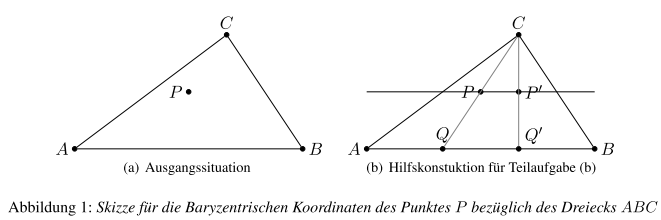
\includegraphics[scale=0.6]{15.png}
\end{center}

Die baryzentrischen Interpolation im 2D kann als Hintereinanderausführung von zwei linearen Inteprolationen aufgefasst werden: Schneidet man die Gerade durch $\overline{CP}$ mit der gegenüberliegenden Dreieckskante $\overline{AB}$,
 so erhält man den Hilfspunkt $Q$, der sich wiederum als baryzentrische Interpolation auf der Strecke $AB$ mit den baryzentrischen Koordinaten $(\alpha',\beta')$ ausdrücken lässt:

2D中的重心插值可以理解为一个接一个的两个线性积分的执行:如果通过CP与直线的相交与相对的三角形边AB,则得到辅助点Q,它又是距离AB上的重心插值,重心坐标为$(\alpha',\beta')$表示:
$$Q=\alpha'A+\beta'B=(1-\beta')A+\beta'B=\alpha'A+(1-\alpha')B$$

Es gilt nun:
$$P=(1-\gamma)Q+\gamma C$$

Entsprechend der linearen Interpolation entlang der Strecke $\overline{QC}$ kann $\gamma$ also bestimmt werden als das Verhältnis der Länge der Teilstrecke $\overline{QP}$ zur Länge der Gesamtstrecke $\overline{QC}$:

因此,与沿着线段QC的线性插值相对应,可以将$\gamma$确定为部分线段QP的长度与总线段QC的长度之比:
$$\gamma = \frac{|P-Q|}{|C-Q|}$$

Die Baryzentrischen Koordinaten im Dreieck werden jedoch zumeist als Verhältnis von Flächeninhalten bzgl. der durch den Punkt aufgespannten Teildreiecke berechnet:

但是,三角形中的重心坐标大部分是根据面积内容与该点所跨越的子三角形的比率来计算的:
$$\alpha = \frac{A_{BCP}}{A_{ABC}},\,\beta=\frac{A_{APC}}{A_{ABC}},\,\gamma=\frac{A_{ABP}}{A_{ABC}}$$

Es kann also auf die Hilfskonstruktionen mit dem Punkt auf der gegenüberliegenden Dreieckskante komplett verzichtet werden.

因此,可以完全省去具有在相对的三角形边缘上的点的辅助构造。
\\
\\
\noindent\textbf{Aufgabe:} Beweisen Sie Gleichung (5) beispielhaft für $\gamma$, indem Sie zeigen, dass gilt:
$$\frac{A_{ABP}}{A_{ABC}}=\frac{|P-Q|}{|C-Q|}$$

Hinweise: 

$\cdot$ Orientieren Sie sich an der Hilfskonstruktion aus Abbildung 1(b).  

$\cdot$ Der Flächeninhalt $A_\Delta$ eines Dreiecks kann als $\frac{1}{2}g\cdot h$ berechnet werden, 
 wobei $g$ der Länge der Grundseite und $h$ der Höhe des Dreiecks (d.h. dem euklidischen Abstand zwischen der durch die Grundseite definierten Geraden und dem dritten Punkt des Dreiecks) entspricht.
\\
\\
\noindent\textbf{2. Flächeninhalt von Dreiecken 三角形面积}

Die Berechnung des Flächeninhaltes über die Formel $\frac{1}{2}g\cdot h$ erweist sich bei allgemeinen Dreiecken sehr umständlich, da zunächst die Höhe bestimmt werden muss. Für ein Dreieck ABC im 2D mit den Eckpunkten
$A=\begin{pmatrix}
    A_x\\A_y
\end{pmatrix},\,B=\begin{pmatrix}
    B_x\\B_y
\end{pmatrix}$ und $C=\begin{pmatrix}
    C_x\\C_y
\end{pmatrix}$ wurde in der Vorlesung eine Formel zur Berechnung des Flächeninhalts vorgestellt, die ohne diese Hilfsberechnungen auskommt. Wir bestimmen (o.E.d.A.) die beiden Vektoren s und t, die ausgehend vom Punkt A das Dreieck aufspannen:

事实证明,使用公式计算面积对于一般三角形非常费力,因为必须首先确定高度。对于具有顶点A B C的2D三角形ABC,在讲座中提出了一个计算面积的公式,该公式无需这些辅助计算即可工作。 我们确定(o.E.d.A.)两个向量s和t,它们从A点开始跨越三角形:

$$s=\begin{pmatrix}
    s_x\\s_y
\end{pmatrix}=B-A=\begin{pmatrix}
    B_x-A_x\\B_y-A_y
\end{pmatrix}$$
$$t=\begin{pmatrix}
    t_X\\t_y
\end{pmatrix}=C-A=\begin{pmatrix}
    C_x-A_x\\C_y-A_y
\end{pmatrix}$$

Dann berechnet sich der Flächeninhalt des Dreiecks als die Determinante einer Matrix mit den Spalten $s$ und $t$:

然后将三角形的面积计算为具有s和t列的矩阵的行列式:

\begin{equation}
    \begin{aligned}
        A_{ABC} =& \frac{1}{2}det\begin{pmatrix}
            s_x & t_x\\s_y&t_y
        \end{pmatrix}=\frac{1}{2}\begin{vmatrix}
            s_x & t_x\\s_y&t_y
        \end{vmatrix}=\frac{1}{2}(s_xt_y-t_xs_y)\\
        A_{ABC} =& \frac{1}{2}\begin{vmatrix}
            B_x-A_x & C_x-A_x\\ B_y-A_y & C_y-A_y
        \end{vmatrix}=\frac{1}{2}[(B_x-A_x)\cdot(C_y-A_y)-(C_x-A_x)\cdot(B_y-A_y)]
    \end{aligned}
\end{equation}

\begin{center}
    
\includegraphics[scale=0.6]{16.png}
\end{center}

Zeigen Sie außschließlich unter Verwendung der Gleichungen $A_\Delta=\frac{1}{2}g\cdot h$ sowie des Flächeninhalts für Rechtecke, dass $A_{ABC}=\frac{1}{2}(s_xt_y-t_xs_y)$ gilt!
Orientieren Sie sich an der Skizze in Abbildung 2(c). (6 Punkte)

仅使用方程式$A_\Delta$和矩形区域即可显示$A_{ABC}$成立! 使用图2(c)中的草图作为指导。
\\
\\
\noindent\textbf{3. Baryzentrische Koordinaten im Dreieck 三角形中的重心坐标}

Gegeben ist das Dreieck ABC und ein Punkt D mit $A=\begin{pmatrix}
    -6\\1
\end{pmatrix},\,B=\begin{pmatrix}
    4\\-1
\end{pmatrix},\,C=\begin{pmatrix}
    2\\5
\end{pmatrix}$ und $D=\begin{pmatrix}
    1\\1
\end{pmatrix}$. Berechnen Sie die baryzentrischen Koordinaten des Punktes $D$ bezüglich des Dreiecks $ABC$!

给定的是三角形ABC以及带有D B和C的点D。计算点D相对于三角形ABC的重心坐标!
\\
\\
\noindent\textbf{4. Anwendung der baryzentrischen Koordinaten 重心坐标的应用(8 Punkte)}

Gegeben sei das folgende Dreieck $ABC$ und die Punkte $P, Q, R$ und $S$.

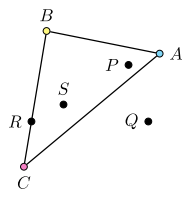
\includegraphics[scale=0.6]{17.png}

\indent\textbf{(a)} Ordnen Sie den Punkten $P, Q, R$ und $S$ die folgenden absoluten baryzentrischen Koordinaten bzgl. des Dreiecks $ABC$ zu:
$W_1=(\frac{3}{4},\frac{1}{8},\frac{1}{8}),\,W_2=(\frac{1}{4},\frac{1}{4},\frac{1}{2}),\,W_3=(1,-\frac{1}{2},\frac{1}{2}),\,W_4=(0,\frac{1}{3},\frac{2}{3})$ (4p)
将相对于三角形ABC的以下绝对重心坐标分配给点P,Q,R和S:

\indent\textbf{(b)} Existieren Punkte für welche alle drei absoluten baryzentrischen Koordinaten negative Werte annehmen? Begründen Sie Ihre Antwort! (2 Punkte)
是否存在所有三个绝对重心坐标都为负的点? 解释你的回答!

\indent\textbf{(c)} Den Eckpunkte des Dreiecks seien die RGB-Farbvektoren $c_A=(0\,\frac{1}{2}\,\frac{5}{6})^T,\,c_B=(1\,1\,0)^T$ und $c_C=(1\,0\,1)^T$ zugeordnet. Berechnen Sie den Farbwert des Punktes $P$ mittels baryzentrischer Interpolation! (2 Punkte)

让RGB颜色矢量cA cB cC分配给三角形的拐角点。 使用重心插值计算点P的颜色值!
\\
\\
\noindent\textbf{PVL 4 - Antwort}

\indent\textbf{1.}
$$A_{ABP} = \frac{1}{2} \cdot  |\overline{AB}| \cdot |\overline{P^{'}Q^{'}}|$$
$$A_{ABC} = \frac{1}{2} \cdot  |\overline{AB}| \cdot |\overline{CQ^{'}}|$$
$$\frac{A_{ABP}}{A_{ABC}} = \frac{|\overline{P^{'}Q^{'}}|}{|\overline{CQ^{'}}|} = \frac{|PQ|}{|CQ|}$$
$$\Rightarrow \frac{A_{ABP}}{A_{ABC}} = \frac{|P-Q|}{|C-Q|}$$


\indent\textbf{2.}
\begin{align*}
    A_{ABC} &= S_x \cdot t_y - A_1 - A_2 - A_3 \\
    &= S_x \cdot t_y - \frac{1}{2} \cdot S_x \cdot S_y - \frac{1}{2}(S_x - t_x)(t_y - S_y) \\
    &= \frac{1}{2}(S_xT_y-t_xS_y)
\end{align*}

\indent\textbf{3.}
$$A_{ABC} = \frac {1}{2} \cdot 
\begin{vmatrix}
    8 & 10 \\
    4 & -2
\end{vmatrix} = 28$$
$$
A_{CDB} = \frac {1}{2} \cdot 
\begin{vmatrix}
    1 & 3 \\
    4 & -2
\end{vmatrix} = 7
$$$$A_{CDA} = \frac {1}{2} \cdot 
\begin{vmatrix}
    1 & -7 \\
    4 & 0
\end{vmatrix} = 14
$$$$A_{ADB} = \frac {1}{2} \cdot 
\begin{vmatrix}
    -7 & 3 \\
    0 & -2
\end{vmatrix} = 7
$$
$$\Rightarrow \alpha = \frac{1}{4} ,\ \beta = \frac{1}{2} ,\ \gamma = \frac{1}{4}$$
$$\Rightarrow D(\frac{1}{4},\ \frac{1}{2},\ \frac{1}{4})$$

\indent\textbf{4.}

\indent\indent\textbf{(a)}

$$W_1 \rightarrow P,\ W_2 \rightarrow S,\ W_3 \rightarrow Q,\ W_4 \rightarrow R$$
\\
\indent\indent\textbf{(b)}

$$\alpha + \beta + \gamma = 1$$\\
\indent\indent Wenn es $\alpha<0,\ \beta<0,\ \gamma<0$ gilt, existiert solche Punkte nicht.
\\

\indent\indent\textbf{(c)}

\indent\indent Laß Ray AP und BC um D treffen.
\indent\indent Denn gilt:

$$D = (1 - \frac{CD}{CB})\cdot c_C + \frac{CD}{CB}\cdot c_B$$
$$P = (1-\frac{AP}{AD})\cdot c_A + \frac{AP}{AD}\cdot D$$
$$P = (\frac{1}{4},\ \frac{1}{2},\ \frac{3}{4})$$

\newpage

\section{PVL 5 - Affine Abbildungen, Transformation des Koordinatensystems}

\noindent\textbf{1. Anwendung affiner Abbildungen 仿射图的应用(7Punkte)}

Gegeben Sei das Rechteck ABCD wie in der Grafik dargestellt (alle Punkte liegen in der Ebene $z$ = 0) sowie die Transformationsmatrix
给定如图所示的矩形ABCD(所有点都位于平面z = 0中)和变换矩阵M。
$M=\begin{pmatrix}
    2&-2&0&1\\
    1&1&0&-5\\
    0&0&-\frac{1}{4}&0\\
    0&0&0&1
\end{pmatrix}$
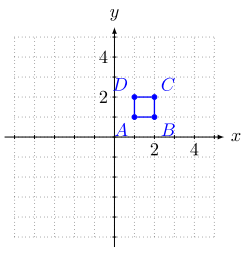
\includegraphics[scale=0.4]{18.png}

\indent\textbf{(a)} Berechnen Sie die Punkte $A'$ bis $D'$, die sich durch die Anwendung der Transformationsmatrix $M$ auf die Punkte $A$ bis $D$ ergeben, und stellen Sie die Abbildung des Rechtecks in der $xy$-Ebene grafisch dar! (4 Punkte)
计算点A到D,这是将变换矩阵M应用于点A到D的结果,并以图形方式表示矩形在xy平面中的表示!

\indent\textbf{(b)} Berechnen Sie die Abbildungen der Einheitsvektoren in $x$- und $y$-Richtung sowie des Koordinatenursprungs, und zeichnen Sie diese ebenfalls in ihre Abbildung aus (a) ein! (3 Punkte)
计算单位向量在x和y方向上的映射以及坐标的原点,并将它们绘制到图片中(a)!
\\
\\
\noindent\textbf{2. Komposition und Umkehrung von affinen Abbildungen 仿射图的合成和反演(14p)}

Gegeben sei eine affine Abbildung M im 3D-Raum, die eine Transformation der Objektpunkte wie in den folgenden Grafiken umsetzt (alle Punkte liegen in der Ebene $z$ = 0):

给定一个3D空间中的仿射映射M,它实现了对象点的转换,如下图所示(所有点都位于平面z = 0中):

\begin{center}
    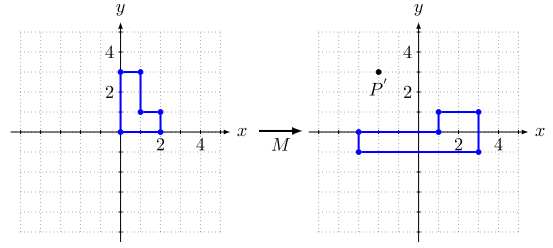
\includegraphics[scale=0.6]{19.png}
\end{center}

\indent\textbf{(a)} Geben Sie eine Sequenz von grundlegenden affinen Abbildungen 
(Rotation, Skalierung, Scherung, Translation) mit ihren Parametern
 (z.B. ,,Rotation um -137$^\circ$ um die y-Achse'',
  ,,Skalierung mit den Faktoren (5, 7, 11)'' etc.) an,
   die hintereinander ausgeführt die Abbildung M ergeben,
   und stellen Sie für jede davon die homogene 4 $\times$ 4-Transformationsmatrix auf! 
   Berechnen Sie schließlich die homogene 4 $\times$ 4 Transformationsmatrix für die Gesamt-Transformation M. (8 Punkte)
   输入带有其参数的一系列基本仿射映射(旋转,缩放,剪切,平移)(例如“绕y轴旋转-137$^\circ$”,“缩放因子(5、7、11)”等) 当一个接一个地执行时,给出映射M,并为每个映射建立均匀的4$\times$4变换矩阵! 最后为整体变换M计算齐次4$\times$4变换矩阵。


\indent\textbf{(b)} Berechnen Sie die homogene 4$\times$4-Transformationsmatrix für die Umkehr-Abbildung $M^{−1}$! Berechnen Sie damit schießlich das Urbild des Punktes $P'$! (6 Punkte)
计算逆映射$M^{-1}$!的齐次4$\times$4变换矩阵!最后,计算点$P'$!的原型。
\\
\\
\noindent\textbf{3. Transformation des Koordinatensystems (4 Punkte)}

Wir betrachten ein Koordinatensystem $K$,
 dass bezüglich unseres Standard-Koordinatensystems gegeben ist als der Ursprungspunkt $O'$
 sowie die Vektoren der Kooridnatenachsen $x', y'$ und $z'$, 
 wie in der Grafik dargestellt. Die $z$-Dimension soll dabei unverändert bleiben, d.h. $z'=z=\begin{pmatrix}
     0\\0\\1\\0
 \end{pmatrix}$ 
 
 如图所示,我们将相对于我们的标准坐标系给出的坐标系K作为原点O'和坐标轴x',y'和z'的向量。 z维度应保持不变,即z'=z

 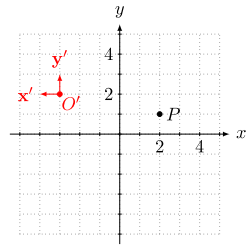
\includegraphics[scale=0.6]{20.png}

 Berechnen Sie die homogene 4 $\times$ 4-Transformationsmatrix der affinen Abbildung,
  die Koordinaten aus unserem Standard-KOS in das KOS $K$ = \{$O',x',y',z'$\} transformiert, 
  und berechnen Sie damit die Koordinaten von $P$ bezüglich $K$!

  计算仿射映射的齐次4$\times$4变换矩阵,该变换矩阵将我们的标准KOS的坐标转换为KOS $K = \{O',x',y',z'\}$,从而计算相对于P的坐标 K!
\\
\\
\noindent\textbf{PVL 5 - Antwort}

\indent\textbf{1.}

\indent\indent\textbf{(a)}
$$A' = M\cdot\begin{pmatrix} 1 \\ 1 \\ 0 \\ 1 \end{pmatrix} =\begin{pmatrix} 1 \\ -3 \\ 0 \\ 1 \end{pmatrix} $$

$$B' = M\cdot\begin{pmatrix} 2 \\ 1 \\ 0 \\ 1 \end{pmatrix} =\begin{pmatrix} 3 \\ -2 \\ 0 \\ 1 \end{pmatrix} $$

$$C' = M\cdot\begin{pmatrix} 2 \\ 2 \\ 0 \\ 1 \end{pmatrix} =\begin{pmatrix} 1 \\ -1 \\ 0 \\ 1 \end{pmatrix} $$

$$D' = M\cdot\begin{pmatrix} 1 \\ 2 \\ 0 \\ 1 \end{pmatrix} =\begin{pmatrix} -1 \\ -2 \\ 0 \\ 1 \end{pmatrix} $$

\indent\indent\textbf{(b)}
$$\vec{e_{x}'} = normiert(M\cdot \vec{e_{x}}) = \frac{1}{5}\cdot \begin{pmatrix} 3 \\ -4 \\ 0 \\ 1 \end{pmatrix}$$

$$\vec{e_{y}'} = normiert(M\cdot \vec{e_{y}}) = \frac{1}{\sqrt{17}}\cdot \begin{pmatrix} -1 \\ -4 \\ 0 \\ 1 \end{pmatrix}$$

$$\vec{e_{z}'} = normiert(M\cdot \vec{e_{z}}) = \frac{4}{\sqrt{417}}\cdot \begin{pmatrix} 1 \\ -5 \\ -\frac{1}{4} \\ 1 \end{pmatrix}$$

$$P' = M\cdot \begin{pmatrix} 0 \\ 0 \\ 0 \\ 0 \end{pmatrix} = \begin{pmatrix} 1 \\ -5 \\ 0 \\ 1 \end{pmatrix}$$

\indent\textbf{2.}

\indent\indent\textbf{(a)} Skalier mit den Faktoren (1,2,1), dreh um $90^{\circ}$ um die Z-Achse, translatier mit dem Vektor(3,-1,0)$^T$:  
$$M_1 = \begin{pmatrix} 1 & 0 & 0 & 0 \\ 0 &2&0&0\\ 0&0&1&0 \\ 0&0&0&1 \end{pmatrix}, M_2 = \begin{pmatrix} cos90^{\circ} & -sin90^{\circ} & 0 & 0 \\ sin90^{\circ} &cos90^{\circ}&0&0\\ 0&0&1&0 \\ 0&0&0&1 \end{pmatrix}, M_3 = \begin{pmatrix} 1 & 0 & 0 & -3 \\ 0 &1&0&-1\\ 0&0&1&0 \\ 0&0&0&1 \end{pmatrix}$$

$$M = M_1 \cdot M_2 \cdot M_3 = \begin{pmatrix} 0 & -2 & 0 & 3 \\ 1 &-2&0&-1\\ 0&0&1&0 \\ 0&0&0&1 \end{pmatrix}$$

\indent\indent\textbf{(b)}
$$M^{-1} = \frac{Adj.A}{det(A)} = \begin{pmatrix} -1 & 1 & 0 & 4 \\ -\frac{1}{2} &0&0&\frac{3}{2}\\ 0&0&1&0 \\ 0&0&0&1 \end{pmatrix}$$ 

$$P = M^{-1}\cdot P' = \begin{pmatrix} 3 \\ \frac{5}{2} \\ 0 \\ 1 \end{pmatrix}$$

\indent\textbf{3.}

$$M^{-1} = \begin{pmatrix} -1 & 0 & 0 & -3 \\ 0 &1&0&2\\ 0&0&1&0 \\ 0&0&0&1 \end{pmatrix}, M =\begin{pmatrix} -1 & 0 & 0 & -3 \\ 0 &1&0&-2\\ 0&0&1&0 \\ 0&0&0&1 \end{pmatrix}$$

$$P' = M \cdot P = \begin{pmatrix} -5\\-1\\0\\1 \end{pmatrix}$$

\newpage

\section{PVL 6 - Projektionsmatrizen, symmetrischen View Frustums, Wirkungen von Projektionen}


\noindent\textbf{1. Projektionsmatrizen 投影矩阵(16 Punkte)}

Gegeben seien die Punkte A bis F mit den Eye-Space-Koordinaten:
$$A=\begin{pmatrix}
    -\frac{9}{5}\\-\frac{9}{10}\\-\frac{9}{5}
\end{pmatrix},\,B=\begin{pmatrix}
    \frac{9}{5}\\-\frac{9}{10}\\-\frac{9}{5}
\end{pmatrix},\,C=\begin{pmatrix}
    \frac{9}{5}\\\frac{9}{10}\\-\frac{9}{5}
\end{pmatrix},\,D=\begin{pmatrix}
    -\frac{9}{5}\\\frac{9}{10}\\-\frac{9}{5}
\end{pmatrix},\,E=\begin{pmatrix}
    -\frac{9}{5}\\-\frac{9}{10}\\-9
\end{pmatrix},\,F=\begin{pmatrix}
    \frac{9}{5}\\-\frac{9}{10}\\-9
\end{pmatrix} $$

sowie die damit beschriebenen Rechtecke $ABCD$ und $ABFE$.

Es sollen zwei Fälle betrachtet werden:

\textbf{A:} Orthogonalprojektion mit den Parametern: $l= -\frac{9}{2},\,r= \frac{9}{2},\,b= -\frac{9}{4},\,t= \frac{9}{4},\,n=1,\,f=9$

\textbf{B:} Zentralprojektion mit den Parametern: $l=-1,\,r=1,\,b=-\frac{1}{2},\,t=\frac{1}{2},\,n=1,\,f=9$

\indent\textbf{(a)} In den Abbildungen auf den nachfolgenden Seiten sind jeweils die Punkte / Rechtecke im $Eye Space$ dargestellt (Draufsicht, d.h. $xz$-Ebene, sowie Seitenansicht von rechts, d.h. $yz$-Ebene). Ergänzen Sie in den Skizzen für die Fälle \textbf{A} und \textbf{B} jeweils das Sichtvolumen, das durch die gegebenen Parameter beschrieben wird! (4 Punkte)
下页的图显示了眼睛空间中的点/矩形(俯视图,即xz平面,右侧视图,即yz平面)在案例A和B的草图中,添加了视觉空间 由给定的参数来描述!

\indent\textbf{(b)} Stellen Sie die Projektionsmatrizen $P_A$ und $P_B$ auf, die sich entsprechend der Fälle \textbf{A} und \textbf{B} ergeben! (2 Punkte)
根据情况A和B设置投影矩阵PA和PB!

\indent\textbf{(c)} Berechnen Sie für die Fälle \textbf{A} und \textbf{B} jeweils die normalisierten Gerätekoordinaten der Punkte \textit{A} bis \textit{F}! (6 Punkte)
计算案例A和案例B的点A到F的标准化设备坐标!

\indent\textbf{(d)} Auf den nachfolgenden Seiten sind ebenfalls Skizzen für den $Normalized Device Space$, jeweils in der Frontansicht ($xy$-Ebene), sowie in der Draufsicht ($xz$-Ebene), vorbereitet. Zeichnen Sie für die Fälle \textbf{A} und \textbf{B} jeweils das Sichtvolumen sowie die Abbildungen der Punkte \textit{A} bis \textit{F} ein! (4 Punkte)
在接下来的页面中,还准备了标准化设备空间的草图,包括正视图(xy平面)和顶视图(xz平面)。 对于情况A和B,请绘制视觉体积以及点A至F的插图。
\\
\\
\noindent\textbf{2. Parametrisierung eines symmetrischen View Frustums 对称视图视锥的参数化(3p)}

Die Spezifikation des View-Frustums über die 6 Parameter $l, r, b, t, n$ und $f$ ist meist sehr unintuitiv. Im Falle einer perspektivischen Projektion mit einem symmetrischen Frustum (d.h. wenn der Betrachter mittig vor der Projektionsfläche platziert ist, was im Normalfall angenommen wird) wird das Sichtvolumen meist durch 4 intuitivere Parameter beschrieben:

通过6个参数l,r,b,t,n 和 f来指定视锥的视图非常不直观。 对于具有对称视锥面的透视投影(即通常将观看者放置在投影表面前面的中央位置,通常是假定的),通常用4个更直观的参数来描述视觉体积:

\indent\indent $\circ$ dem Seitenverhältnis $a$, d.h. dem Verhältnis $\frac{Breite}{Hoehe}$ der Fläche, auf der das Bild ausgegeben werden soll,

\indent\indent $\circ$ dem \textbf{vertikalen} Öffnungswinkel $\theta$ (engl. \textit{field ofview angle} bzw. kurz \textit{FOV}),

\indent\indent $\circ$ dem Abstand $n$ zur Near-Plane (in Blickrichtung) und

\indent\indent $\circ$ dem Abstand $f$ zur Far-Plane (in Blickrichtung).

Aus diesen Parametern können die 6 Parameter für ein allgemeines View Frustum bestimmt werden.

可以从这些参数中确定用于普通视锥的6个参数。

Es soll eine Projektionsmatrix erstellt werden,
 die eine unverzerrte Ausgabe für ein Fenster aus 720 $\times$ 480 Pixeln erzeugt. 
 Der Öffnungswinkel betrage $\theta=90^\circ$. 
 Die Near-Plane soll $n$ = 2 Einheiten vor dem Betrachter liegen, 
 und die Far Plane $f$ = 32 Einheiten.

将创建一个投影矩阵,为720$\times$480像素的窗口产生不失真的输出。 张开角为$\theta$= 90$^\circ$。 近平面在观看者面前应该为n = 2个单位,远平面f = 32个单位。

Bestimmen Sie die Parameter $l, r, b, t$ für das allgemeine View Frustum, dass sich aus den gegebenen Parametern ergibt!
\\
\\
\noindent\textbf{3. Wirkungen von Projektionen 投影效果(6 Punkte)}

Gegeben sei ein achsparalleler Einheitswürfel in 3D, der in die 2D-$xy$-Ebene projiziert wird.
 Geben Sie für jeden der folgenden Fälle an, ob die beschriebene Situation mit einer Otrhogonalprojektion und ob die beschriebene Situation mit einer Zentralprojektion möglich ist:

给定投影到2D xy平面中的3D轴向平行的单位立方体,请针对以下每种情况说明以下情况:正交投影可能导致上述情况发生,而中心投影可能导致上述情况发生:

\indent\textbf{(a)} Die 2D-Abbildungen aller Kanten, die parallel zur Projektionsebene liegen, sind gleich lang.
平行于投影平面的所有边缘的2D图像的长度相同。

\indent\textbf{(b)} Die 2D-Abbildungen aller Seitenflächen, die parallel zur Projektionsebene liegen, sind Quadrate.
平行于投影平面的所有侧面的2D图像均为正方形。

\indent\textbf{(c)} Die Flächeninhalt der Abbildung einer Seitenfläche, die senkrecht zur Projektionsebene liegt, ist nicht 0. Begründen Sie Ihre Antworten!
垂直于投影平面的侧面图像的面积不为0.请给出答案!

\noindent\textbf{PVL 6 - Antwort}

\indent\textbf{1.}

\indent\indent\textbf{(b)}
$$
P_A = 
\begin{pmatrix}
    \frac{2}{9} & 0 & 0 & 0 \\
    0 & \frac{4}{9} & 0 & 0 \\
    0 & 0 & \frac{1}{4} & -\frac{5}{4} \\
    0 & 0 & 0 & 1
\end{pmatrix}, 
P_B =
\begin{pmatrix}
    1 & 0 & 0 & 0 \\
    0 & 2 & 0 & 0 \\
    0 & 0 & -\frac{5}{4} & -\frac{9}{4} \\ 
    0 & 0 & -1 & 0
\end{pmatrix}
$$

\indent\indent\textbf{(c)}
I: $A' = P_A \cdot A $

$$A' = 
\begin{pmatrix}
    \frac{2}{9} & 0 & 0 & 0 \\
    0 & \frac{4}{9} & 0 & 0 \\
    0 & 0 & -\frac{1}{4} & -\frac{5}{4} \\
    0 & 0 & 0 & 1
\end{pmatrix} \cdot
\begin{pmatrix}
    -\frac{9}{5} \\ -\frac{9}{10} \\ -\frac{9}{5} \\ 1  
\end{pmatrix} = 
\begin{pmatrix}
    -\frac{2}{5} \\ -\frac{2}{5} \\ -\frac{4}{5} \\ 1
\end{pmatrix} 
$$
$$
B' =
\begin{pmatrix}
    \frac{2}{5} \\ -\frac{2}{5} \\ -\frac{4}{5} \\ 1
\end{pmatrix}, 
C'=
\begin{pmatrix}
    \frac{2}{5} \\ \frac{2}{5} \\ -\frac{4}{5} \\ 1    
\end{pmatrix}, 
D'=
\begin{pmatrix}
    -\frac{2}{5} \\ \frac{2}{5} \\ -\frac{4}{5} \\ 1    
\end{pmatrix}, 
E'=
\begin{pmatrix}
    -\frac{2}{5} \\ -\frac{2}{5} \\ 1 \\ 1    
\end{pmatrix}, 
F'=
\begin{pmatrix}
    \frac{2}{5} \\ -\frac{2}{5} \\ 1 \\ 1    
\end{pmatrix}
$$

II: $A' = P_B \cdot A $
$$
A'=
\begin{pmatrix}
    -\frac{9}{5} \\ -\frac{9}{5} \\ 0 \\ \frac{9}{5}    
\end{pmatrix},
B'=
\begin{pmatrix}
    \frac{9}{5} \\ -\frac{9}{5} \\ 0 \\ \frac{9}{5}    
\end{pmatrix},
C'=
\begin{pmatrix}
    \frac{9}{5} \\ \frac{9}{5} \\ 0 \\ \frac{9}{5}    
\end{pmatrix},
D'=
\begin{pmatrix}
    -\frac{9}{5} \\ \frac{9}{5} \\ 0 \\ \frac{9}{5}    
\end{pmatrix},
E'=
\begin{pmatrix}
    -\frac{9}{5} \\ -\frac{9}{5} \\ 9 \\ 9    
\end{pmatrix},
F'=
\begin{pmatrix}
    \frac{9}{5} \\ -\frac{9}{5} \\ 9 \\ 9    
\end{pmatrix}
$$

\indent\textbf{2.}

\quad \  $a = \frac{720}{480} = \frac{3}{2}$

\quad \  $t = n \cdot tan(\frac{\theta}{2}) = 2tan(\frac{\pi}{2}) = 2$

\quad \  $r = t \cdot a = 2 \cdot \frac{3}{2} = 3$

\quad \  $l = -r = -3, \ b = -t = -2$


\indent\textbf{3.}

\indent\indent\textbf{(a)} Nur bei Orthogonale Projektion ist es möglich, denn sie parallelprojektion ist, dabei sind all Kanten auf 2D-Abbildung gleich lang.

\indent\indent\, Dagegen ist es bei zentrale Projektion aufgrund ihrer Differenz der Distanz zweischen verschiedene Kanten und Ursprung nicht möglich.

\indent\indent\textbf{(b)} Beide sind möglich. Darunter muss die Ursprung (bei Orthogonale Projektion) sich in der Zentrum der Seite befinden.

\indent\indent\textbf{(c)} Nur bei Zentrale Projektion ist es möglich, denn die obene- und untere Edge der Seite auf der Projektionsebene nicht aufeinander, ist die Flächeinheit nicht 0.

\indent\indent\, Bei Orthogonale Projektion: Wenn die Seiten senkrecht zur Projektionsebene ist, ist die Abbildung der Seite eine Gerade, deswegen nicht möglich.

(a)只有正交投影才有可能,因为它是平行投影,并且二维地图上的所有边长都相同。

\indent\indent\,相反,在中心投影的情况下,由于两个不同的边缘和原点之间的距离不同而无法实现。

(b)两者都是可能的。 在此之下,原点(用于正交投影)必须位于页面的中心。

(c)仅在中心投影时才有可能,因为投影平面上侧面的上下边缘不重叠,所以面积单位不为0。

\indent\indent\,对于正交投影:如果该侧面垂直于投影平面,则该侧面将显示为直线,因此是不可能的。

\includepdf[pages={2,3,4}]{CG1-PVL6-DongzeYang-comp.pdf}

\newpage

\section{PVL 7 - Koordinatentransformation}

\noindent\textbf{1. Koordinatentransformation (24p)}

Wir betrachten ein Dreieck $ABC$, dessen Koordinaten im \textit{Object Space} gegeben seien als:

$$A_{obj}=\begin{pmatrix}
    -1\\0\\0
\end{pmatrix},\,B_{obj}=\begin{pmatrix}
    1\\0\\0
\end{pmatrix},\,C_{obj}=\begin{pmatrix}
    0\\1\\0
\end{pmatrix}$$

Weiterhin seien die Model-Matrix $M$ und die Projektions-Matrix $P$ gegeben:

$$M=\begin{pmatrix}
    0&8&0&6\\
    0&0&1&-2\\
    4&0&0&0\\
    0&0&0&1
\end{pmatrix},\,P=\begin{pmatrix}
    1&0&0&0\\
    0&2&0&0\\
    0&0&-2&-12\\
    0&0&-1&0
\end{pmatrix}$$

Die Kamera sei bezüglich des \textit{World Space} beschrieben: Sie befinde sich am Punkt $\begin{pmatrix}
    2\\0\\0
\end{pmatrix}$, ihre lokale $x$-Achse zeigt in Richtung $\begin{pmatrix}
    0\\0\\1
\end{pmatrix}$, ihre $y$-Achse in Richtung $\begin{pmatrix}
    0\\1\\0
\end{pmatrix}$ und ihre $z$-Achse in Richtung $\begin{pmatrix}
    -1\\0\\0
\end{pmatrix}$. Das Ausgabe-Fenster sei 32$\times$18 Pixel groß, als Viewport werde ein 16$\times$12 Pixel großer Bereich gewählt, der am Pixel
$\begin{pmatrix}
    4\\4
\end{pmatrix}$ beginne. Der sichtbare Tiefenbereich werde im \textit{Window Space} auf das Intervall [0, 1] abgebildet.

(Es gelten alle Konventionen zu Koordinatensystemen und Sichtvolumen, wie Sie in der Vorlesung vorgestellt wurden. 如讲座中所述,适用于坐标系和视觉体积的所有约定。)

\indent\textbf{(a)} Berechnen Sie die View-Matrix $V$, die die gegebene Kamera-Position und Orientierung umsetzt! (4 Punkte)
计算视图矩阵V,该矩阵实现给定的相机位置和方向!

\indent\textbf{(b)} Berechnen Sie die Koordinaten der Punkte $A, B$ und $C$ bezüglich der folgenden Räume: (10 Punkte)

\indent\indent - Clip Space 

\indent\indent - Eye Space 

\indent\indent - Normalized Device Space 

\indent\indent - World Space

\indent\textbf{(c)} Berechnen Sie die Window-Space-Koordinaten der Punkte $A$ bis $C$.
 In der Skizze unten ist der Window Space für das Fenster in der Frontansicht ($xy$-Ebene, 
 d.h. die tatsächliche Abbildung, wie sie später auf dem Monitor erscheinen soll) dargestellt. Ergänzen Sie dort den Viewport sowie die Abbildung des Dreiecks $ABC$! (5 Punkte)
 计算点A到C的窗口空间坐标。下面的草图在前视图(xy平面,即稍后应在监视器上显示的实际图像)中显示了窗口的窗口空间。 在此添加视口和三角形ABC的插图!

\indent\textbf{(d)} Geben Sie ein Verfahren an, mit den Sie für einen beliebigen Punkt mit bekannten Eye-SpaceKoordinaten
$X_{eye}=\begin{pmatrix}
    x_{eye}\\y_{eye}\\z_{eye}
\end{pmatrix}$ bestimmen können, ob der Punkt innerhalb oder außerhalb des Sichtvolumens liegt! Bestimmen Sie damit, ob die Punkte $Q, R$ und $S$ innerhalb oder außerhalb des Sichtvolumens
liegen 给出一种方法,您可以使用该方法确定具有已知眼空间坐标$X_{eye}$的任何点,该点是在视觉体积之内还是之外! 使用它来确定点Q,R和S在可见体积之内还是之外: $Q_{eye}=\begin{pmatrix}
    -1\\-1\\-6
\end{pmatrix},\,R_{eye}=\begin{pmatrix}
    -1\\-1\\0
\end{pmatrix}$ und $S_{eye}=\begin{pmatrix}
    -1\\-1\\6
\end{pmatrix}$!

\begin{center}
    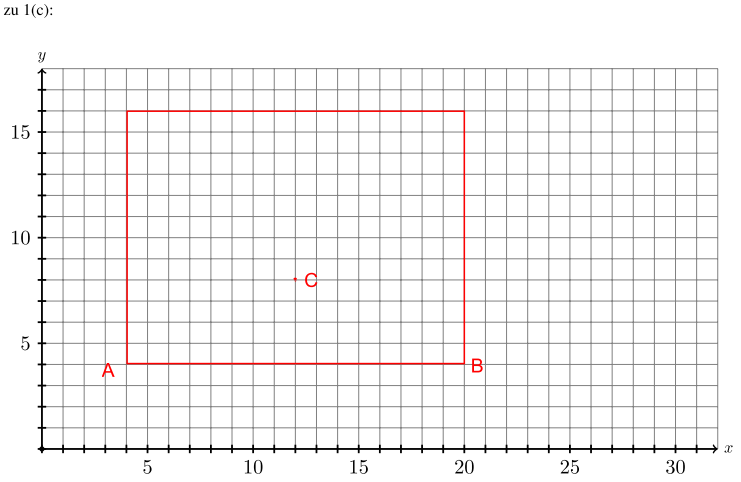
\includegraphics[scale=0.6]{21.png}
\end{center}

\noindent\textbf{PVL 7 - Antwort}

\indent\textbf{(a)}
$$V = 
\begin{pmatrix}
    0 & 0 & 1 & 0 \\
    0 & 1 & 0 & 0 \\
    -1 & 0 & 0 &0 \\
    0 & 0 & 0 & 1
\end{pmatrix} \cdot
\begin{pmatrix}
    1 & 0 & 0 & -2 \\
    0 & 1 & 0 & 0 \\
    0 & 0 & 1 & 0 \\
    0 & 0 & 0 & 1
\end{pmatrix} = 
\begin{pmatrix}
    0 & 0 & 1 & 0 \\
    0 & 1 & 0 & 0 \\
    -1 & 0 & 0 & 2 \\
    0 & 0 & 0 & 1
\end{pmatrix}
$$

\indent\textbf{(b)}
$$A_{ws} = M \cdot A_{obj} = M \cdot \begin{pmatrix} -1 \\ 0 \\ 0 \\ 1 \end{pmatrix} = \begin{pmatrix} 6 \\ -2 \\ -4 \\ 1 \end{pmatrix}$$
$$B_{ws} = M \cdot B_{obj} = \begin{pmatrix} 6 \\ -2 \\ 4 \\ 1 \end{pmatrix}$$
$$C_{ws} = M \cdot C_{obj} = \begin{pmatrix} 14 \\ -2 \\ 0 \\ 1 \end{pmatrix}$$
\\
$$A_{es} = V \cdot M \cdot A_{obj} = P \cdot A_{ws} =  \begin{pmatrix} -4 \\ -2 \\ -4 \\ 1 \end{pmatrix}$$
$$B_{es} = P \cdot B_{ws} =  \begin{pmatrix} 4 \\ -2 \\ -4 \\ 1 \end{pmatrix}$$
$$C_{es} = P \cdot C_{ws} =  \begin{pmatrix} 0 \\ -2 \\ -12 \\ 1 \end{pmatrix}$$
\\
$$A_{cs} = P \cdot V \cdot M \cdot A_{obj} = P \cdot A_{es} = \begin{pmatrix} -4 \\ -4 \\ -4 \\ 4 \end{pmatrix}$$
$$B_{cs} = P \cdot B_{es} = \begin{pmatrix} 4 \\ -4 \\ -4 \\ 4 \end{pmatrix}$$
$$C_{cs} = P \cdot C_{es} = \begin{pmatrix} 0 \\ -4 \\ 12 \\ 12 \end{pmatrix}$$
\\
$$A_{nds} = \frac{1}{4} \cdot A_{cs} = \begin{pmatrix} -1 \\ -1 \\ -1 \\ 1 \end{pmatrix}$$
$$B_{nds} = \frac{1}{4} \cdot B_{cs} = \begin{pmatrix} 1 \\ -1 \\ -1 \\ 1 \end{pmatrix}$$
$$C_{nds} = \frac{1}{4} \cdot C_{cs} = \begin{pmatrix} 0 \\ -\frac{1}{3} \\ 1 \\ 1 \end{pmatrix}$$

\indent\textbf{(c)}
$$A = 
\begin{pmatrix}
    8 & 0 & 0 & 12 \\
    0 & 6 & 0 & 10 \\
    0 & 0 & \frac{1}{2} & \frac{1}{2} \\
    0 & 0 & 0 & 1
\end{pmatrix}
$$
$Window-Space-Koordinaten = A \cdot Punkte_{nds}$
$$A_{wsk} = \begin{pmatrix} 4 \\ 4 \\ 0 \\ 1 \end{pmatrix}
B_{wsk} = \begin{pmatrix} 20 \\ 4 \\ 0 \\ 1 \end{pmatrix}
C_{wsk} = \begin{pmatrix} 12 \\ 8 \\ 1 \\ 1 \end{pmatrix}$$
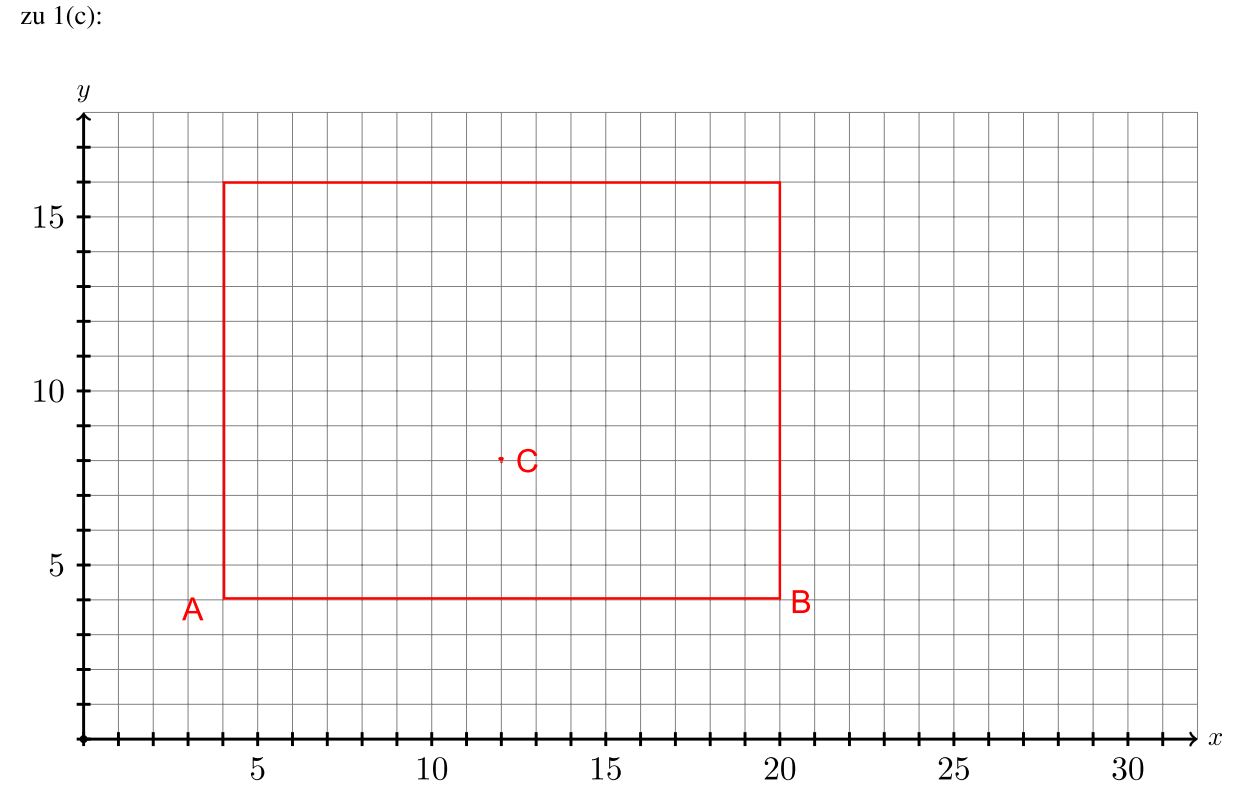
\includegraphics[scale=0.3]{QQ截图20200114020456.png}

\indent\textbf{(d)}

$Punkte_{cs} = P \cdot Punkte_{es}, \
Punkte_{nds} = normalisiert(Punkte_{cs})$

Außerhalb, wenn ein Wert in $Punkte_{nds}$ größer als 1 oder kleiner als -1 ist, sonst innerhalb.

gilt:

$Q_{es}$: innerhalb, $R_{es}$: Außerhalb, $S_{es}$: Außerhalb

\newpage

\section{PVL 8 - Umkehrung der Koordinatentransformation, Tiefentest und Projektionsmatrizen, Tiefentest in der Renderpipeline}

\noindent\textbf{1. Umkehrung der Koordinatentransformation 坐标变换的逆(13p)}

Wir betrachten ein polygonales Objekt, dass innerhalb der $xy$-Ebene im \textit{Object Space} liege.
 Dieses Objekt werde mit der Render-Pipeline dargestellt. 

 我们考虑一个位于对象空间xy平面内的多边形对象。 该对象用渲染管道表示。

Es sei die Koordinaten-Transformation in Form der Matrizen $M, V$ und $P$ sowie ihrer Inversen bekannt:
让坐标变换以矩阵M,V和P以及它们的逆的形式知道:

$$M=\begin{pmatrix}
    0&-1&0&0\\
    1&0&0&0\\
    0&0&-1&2\\
    0&0&0&1
\end{pmatrix},\,V=\begin{pmatrix}
    0&0&1&0\\
    0&-1&0&0\\
    -1&0&0&2\\
    0&0&0&1
\end{pmatrix},\,P=\begin{pmatrix}
    1&0&0&0\\
    0&2&0&0\\
    0&0&-\frac{3}{2}&-5\\
    0&0&-1&0
\end{pmatrix}$$

$$M^{-1}=\begin{pmatrix}
    0&1&0&0\\
    -1&0&0&0\\
    0&0&-1&2\\
    0&0&0&1
\end{pmatrix},\,V^{-1}=\begin{pmatrix}
    0&0&-1&2\\
    0&-1&0&0\\
    1&0&0&0\\
    0&0&0&1
\end{pmatrix},\,P^{-1}=\begin{pmatrix}
    1&0&0&0\\
    0&\frac{1}{2}&0&0\\
    0&0&0&-1\\
    0&0&-\frac{1}{5}&\frac{3}{10}
\end{pmatrix}$$

Es werde ein Fenster mit der (für die Einfachheit der Berechnungen unrealistisch niedrigen)
 Auflösung von 6$\times$6 Pixel verwendet, und der Viewport fülle dieses Fenster exakt aus. Der Tiefenbereich werde so abgebildet, dass die Near Plane bei 0 und die Far Plane bei 1 im Window Space liegen.

 使用分辨率为6$\times$6像素的窗口(为简化计算,该分辨率实在太低了),并且视口正好填充了该窗口。 映射深度范围,以使0处的近平面和1处的远平面位于窗口空间中。

Sei $E$ die $xy$-Ebene im Object Space, d.h. $E$ : $z_{obj}$ = 0.
 Es soll nun angenommen werden, dass der Benutzer mit der Maus auf ein Pixel dieses Fensters klickt, und es soll derjenige Punkt in der Ebene $E$ im Object Space bestimmt werden, der in diesem Pixel abgebildet wurde.

 设E为对象空间中的xy平面,即E:$z_{obj}$ =0。现在应假定用户用M单击此窗口中的一个像素,并确定对象空间中平面E上的那个点。 映射到此像素。

Typische graphische Benutzeroberflächen wie Windows, Qt,
 das X Window System, usw. liefern die Mauskoordinaten als ganzahlige 2D-Koordinaten, 
 wobei der Ursprung des Koordinatensystems dem linken oberen Pixel entspricht. 
 Unsere Renderpipeline verwendet jedoch (analog zu OpenGL) die Konvention 
 mit dem Ursprung \textbf{unten} links. Weiterhin muss berücksichtigt werden, 
 dass im Window Space jedes Pixel durch ein Quadrat der Kantenlänge 1 
 repräsentiert wird. Daher soll angenommen werden, dass 2DMauskoordinaten das 
 Zentrum eines Pixels repräsentieren (das Coverage Sampling bei der 
 Rasterisierung testet ebenfalls jeweils die Pixelzentren und verwendet 
 diese Daten stellvertretend für das gesamte Pixel). Es ist deshalb 
 zunächst eine Transformation vom Maus-Koordinatensystem in den Window Space notwendig.

 典型的图形用户界面,例如Windows,Qt,X Window System等,将鼠标坐标提供为整数2D坐标,坐标系统的原点对应于左上像素。 但是,我们的渲染管道使用(类似于OpenGL)原始左下角的约定。 还必须考虑到,窗口空间中的每个像素都由边长为1的正方形表示。 因此,应假定2D鼠标坐标表示像素的中心(光栅化期间的覆盖率采样还测试相应的像素中心,并将此数据用于整个像素)。 因此,首先需要将鼠标坐标系转换为窗口空间。

In der nebenstehenden Abbildung ist die Situation dargestellt. Die MausKoordinaten repräsentieren ganze Pixel bzgl. des rot eingezeichneten Koordinatenystems (oben und rechts). Beispielhaft ist das Pixel mit den 2D-Mauskoordinaten
$\begin{pmatrix}
     4\\4
 \end{pmatrix}$ dargestellt. Der zugehörige Window-Space-Punkt des Pixelzentrums hat folglich die Koordinaten
$\begin{pmatrix}
    2.5\\4.5\\z_{win}
\end{pmatrix}=\begin{pmatrix}
    \frac{5}{2}\\\frac{9}{2}\\z_{win}
\end{pmatrix}$.

右图显示了情况。 鼠标坐标代表相对于以红色绘制的坐标系统(上方和右侧)的整个像素。 以具有2D鼠标坐标$(4\, 4)^T$的像素为例。 因此,像素中心的关联窗口空间点具有坐标$(\,)$

Der Window-Space ist allerdings dreidimensional und der Wert von $z_{win}$ zunächst unbestimmt.

但是,窗口空间是三维的,并且二维的值最初是不确定的。

\begin{center}
    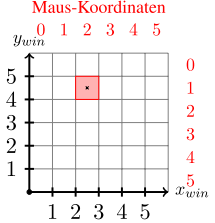
\includegraphics[scale=0.6]{22.png}
\end{center}

Die 2D-$xy$-Koordinaten im Window Space repräsentieren einen Sichtstrahl,
 der durch unsere Szene verläuft. Alle Punkte eines solchen Strahls werden auf 
 die gleiche 2D-Position im Fenster projiziert. Wir können also zwei Punkte 
 $A$ und $B$ angeben, um den Strahl zu definieren, der bei $A$ beginnt und durch den 
 Punkt $B$ verläuft. Zweckmäßig ist es dabei, einen Punkt auf der Near Plane 
 ($z_{win}$ = 0), sowie einen auf der Far Plane ($z_{win}$ = 1) auszuwählen\footnote{Da das Sichtvolumen vorn und hinten begrenzt ist, handelt es sich strenggenommen gar nicht um einen Strahl, sonder schlichtweg um die Strecke $\overline{AB}$, die alle Punkte beschreibt, welche nach dem Clipping auf die jeweilige Window-Space $xy$-Position abgebildet werden. Je nach Anwendungsszenario kann es sinnvoll sein, eine Gerade, einen Strahl beginnend vom Punkt $A$ auf der near Plane, oder die Strecke $\overline{AB}$ für die Schnittpunktberechnungen zu verwenden. In der nachfolgenden Aufgabenstellung soll vereinfachend mit einer komplett unbeschränkten Gerade gerechnet werden, so dass der Schnittpunkt potentiell auch hinter der Kamera liegen könnte. 由于可见体积在前后受到限制,严格来说,它根本不是光线,而只是距离AB,它描述了裁剪后映射到相应窗口空间xy位置的所有点。 根据应用场景,使用直线,从近平面上的点A出发的射线或段AB进行相交计算可能很有意义。 为简单起见,应使用完全不受限制的直线来计算以下任务,以使交点也可能位于相机的后面。}. 
 Es ergeben sich also folgende 3D-Koordinaten im Window Space:

 窗口空间中的2D xy坐标代表贯穿我们场景的一束视觉。 此类射线的所有点都将投影到窗口中相同的2D位置。 因此,我们可以指定两个点A和B来定义从A开始并经过点B的射线。 在近平面(zwin = 0)上选择一个点,在远平面(zwin = 1)上选择一个点很有用。 这将在窗口空间中产生以下3D坐标:

$$A_{win}=\begin{pmatrix}
    \frac{5}{2}\\\frac{9}{2}\\0
\end{pmatrix},\,B_{win}=\begin{pmatrix}
    \frac{5}{2}\\\frac{9}{2}\\1
\end{pmatrix}$$

Diese Punkte können in beliebige Räume zurücktransformiert werden, um den zugehörigen Sichtstrahl im betreffenden Raum zu bestimmen.

这些点可以转换回任何空间,以便确定相关空间中的关联视线。

\indent\textbf{(a)} Berechnen Sie die Koordinaten von $A$ und $B$ im \textit{Normalized Device Space}! (4 Punkte)
计算归一化设备空间中A和B的坐标!

\indent\textbf{(b)} Berechnen Sie die Koordinaten von $A$ und $B$ im \textit{Object Space} (6 Punkte)
计算物体空间中A和B的坐标

\indent\textbf{(c)} Berechnen Sie im Object Space den Schnittpunkt $Q$, der sich ergibt, wenn die Gerade, die durch die Punkte $A$ und $B$ verläuft, mit der gegebenen Ebene $E$ geschnitten wird! (3 Punkte)
计算物体空间中相交点Q,该相交点Q穿过点A和点B的直线与给定平面E相交!
\\
\\
\noindent\textbf{2. Tiefentest und Projektionsmatrizen 深度测试和投影矩阵(7P)}

Gegeben seien die folgenden Projektionsmatrizen:

$$P_1=\begin{pmatrix}
    \frac{5}{6}&0&0&0\\
    0&-1&0&0\\
    0&0&-\frac{3}{2}&-\frac{1}{4}\\
    0&0&0&1
\end{pmatrix},\,P_2=\begin{pmatrix}
    \frac{5}{6}&0&0&0\\
    0&-1&0&0\\
    0&0&-\frac{5}{2}&-3\\
    0&0&-1&0
\end{pmatrix}$$

\indent\textbf{(a)} Geben Sie für jede der Matrizen die Funktion an,
 die die durch sie definierte Abbildung $z_{ndc}(z_{eye})$ beschreibt! 
 (Dabei sei $z_{eye}$ der Tiefenwert im Eye Space und $z_{ndc}$ der Tiefenwert in 
 normalisieren Gerätekoordinaten.) (2 Punkte)
 为每个矩阵提供描述它们定义的映射zndc(zeye)的函数! (让zeye为眼睛空间中的深度值,让zndc为使设备标准化的深度值。)

\indent\textbf{(b)} Für den Tiefentest werde ein Z-Buffer mit 4Bit vorzeichenlosen Ganzzahlen verwendet. Die Überführung des Tiefenwertes von NDC in den Wertebereich des Z-Buffers erfolge gemäß\footnote{Wir gehen dabei implizit davon aus, dass der NDC-Tiefenwert zunächst vom Intervall [−1, 1] auf einen Window-Space-Tiefenwert im Interval [0, 1] transformiert werde, d.h. $z_{win}(z_{ndc}) = \frac{1}{2}(z_{ndc} +1)$ und dieser dann auf den mit 4 Bit darstellbaren Wertebereich $0, 1, . . . , 2^4 − 1$ für den eigenltichen Buffer abgebildet werde: $z_{buf}(z_{win}) = \lfloor(2^4 − 1)z_{win}\rfloor.$}:
具有4位无符号整数的Z缓冲区用于深度测试。 深度值从NDC到Z缓冲区的值范围的传输根据

$$z_{buf}(z_{ndc})=\lfloor\frac{2^4-1}{2}(z_{ndc}+1)\rfloor$$

Der Tiefentest sei so definiert, dass ein Fragment nur gezeichnet wird, wenn sein Tiefenwert echt kleiner ist als der aktuelle Tiefenwert an dieser Stelle im Z-Buffer.

深度测试的定义方式是,仅当片段的深度值确实小于Z缓冲区中当前深度值时才绘制片段。

Beim Rendern entstehe zunächst Fragment $F_1$,
 welches den Tiefentest bestehe.
 Später entstehe für genau diese Pixelposition noch das Fragment $F_2$. 
 Gegeben seien die Werte $z_1$ und $z_2$, welche die $z$-Koordinate von $F_1$ bzw. $F_2$ 
 im Eye Space repräsentieren. Wir betrachten die folgenden 2 Fälle:

 渲染时,结果是片段F1,它通过了深度测试。 稍后将针对该像素位置创建片段F2。 给出值z1和z2,它们表示眼睛空间中F1和F2的z坐标。 我们考虑以下两种情况:

\textbf{A:} $z_1=-3,\,z_2=-2$

\textbf{B:} $z_1=-9,\,z_2=-8$

In beiden Fällen liegt $F_2$ im Eye-Space eine Einheit näher am Betrachter als $F_1$.

在这两种情况下,F1都比F1在眼睛空间中更靠近观看者一个单位.

Für den Fall \textbf{A} ergibt sich

mit $P_1$ für $F_1$ : $z_{buf}(z_{ndc}(z_1))=39$, für $F_2$: $z_{buf}(z_{ndc}(z_2))=28$, d.h. $F_2$ besteht den Tiefentest,

mit $P_2$ für $F_1$ : $z_{buf}(z_{ndc}(z_1))=18$, für $F_2$: $z_{buf}(z_{ndc}(z_2))=15$, d.h. $F_2$ besteht ebenfalls den Tiefentest.

Berechnen Sie für den Fall \textbf{B}, ob $F_2$ den Tiefentest bestehen würde,
 jeweils einmal unter Verwendung von $P_1$ und einmal unter Verwendung von $P_2$! 
 Erklären Sie, beim Einsatz welcher Matrix ein Darstellungsproblem auftritt, und beschreiben Sie dieses Problem kurz. (5 Punkte)

 对于情况B,计算一次F2是否通过深度测试,一次使用P1,一次使用P2! 解释在使用时出现显示问题的矩阵,并简要描述问题。
 \\
\\
\noindent\textbf{3. Tiefentest in der Renderpipeline 渲染管道中的深度测试(5p)}

Wir betrachten einen \textit{Draw Call}, bei dem nacheinander drei Rechtecke $R1,R2$ und $R3$
 (bestehend aus jeweils zwei Dreiecken) gezeichnet werden. 
 Im Object Space seien die Rechtecke alle parallel zur $xy$-Ebene ausgerichtet, 
 lediglich die $z$-Koordinaten der drei Rechtecke unterscheide sich. Als Model-, View- 
 und Projektionsmatrix komme die Einheitsmatrix zum Einsatz, d.h. $M = V = P = I$ 
 und die Object-Space-Koordinaten sind identisch mit den NDC-Koordinaten. 
 Der Viewport entspricht dem gesamten Fenster und die Near Plane werde im Window Space auf 
 $z_{win}$ = 0, die Far-Plane auf $z_{win}$ = 1 abgebildet. 
 Alle drei Rechtecke füllen den Viewport komplett aus. Backface-Culling und Blending sei 
 deaktiviert. Direkt vor dem Draw Call wurde der Color Buffer in jedem Pixel auf 
 schwarz intialisiert, und der Depth Buffer überall auf 1. Der Tiefentest sei aktiviert 
 und auf die Vergleichsrichtung \textbf{kleiner gleich} eingestellt. 
 Der Framebuffer sei 640$\times$480 Pixel groß und wir betrachten das Pixel $p$ mit den Koordinaten 
$p=(400\,\,200)^T$ im Framebuffer.

我们考虑一个绘制调用,其中三个矩形R1,R2和R3(每个由两个三角形组成)一个接一个地绘制。在对象空间中,所有矩形均平行于xy平面对齐,只有三个矩形的z坐标不同。单位矩阵用作模型,视图和投影矩阵,即M = V = P = I,并且对象空间坐标与NDC坐标相同。视口对应于整个窗口,并且在窗口空间中,近平面映射到zwin = 0,远平面映射到zwin = 1。所有三个矩形完全填充了视口。背面剔除和混合禁用。在绘制调用之前,每个像素的颜色缓冲区均初始化为黑色,各处的深度缓冲区均初始化为1,深度测试被激活并设置为小于或等于比较方向。帧缓冲区为640$\times$480像素,我们考虑帧缓冲区中坐标p =$(400\, 200)^T$的像素p。

Während der Ausführung des Draw Calls ergeben sich für das Pixel $p$ eine gewisse Anzahl
 von schreibenden Zugriffen auf den Depth Buffer, und nach dem Draw Call steht im Color 
 Buffer an der Stelle $p$ der Farbwert eines der Rechtecke. Seien $z_1, z_2$ und $z_3$ die 
 \textit{Object Space} $z$-Koordinaten der drei Rechtecke. Diese Werte können innerhalb 
 der folgenden Grenzen gewählt werden: $−1 \leq z_1, z_2, z_3 \leq 1$. Füllen Sie die folgende Tabelle aus:

 在执行绘图调用期间,对像素p的深度缓冲区有一定数量的写访问,并且在绘图调用之后,矩形之一的颜色值在位置p的颜色缓冲区中。 令z1,z2和z3为三个矩形的对象空间z坐标。 可以在以下范围内选择这些值:-1$\leq$z1,z2,z3$\leq$1。 填写下表:

\begin{center}
    \begin{tabular}{|c|c|c|c|c|}
        \hline
        \textbf{\#Schreibzugriffe} & \textbf{sichtbares Rechteck}&\qquad$z_1$\qquad\qquad&\qquad$z_2$\qquad\qquad&\qquad$z_3$\qquad\qquad\\
        \hline
        &&0.5&0.6&-0.2\\
        \hline
        &$R_1$&&&\\
        \hline
        3&&&&\\
        \hline
    \end{tabular}
\end{center}

(In den Fällen, in denen die $z$-Werte nicht vorgeben sind, sollen konkrete Zahlenwerte angegeben werden, die zu der geforderten Situation führen. 在未指定$ z $值的情况下,应指定导致所需情况的特定数值。)
\\
\\
\noindent\textbf{PVL 8 - Antwort}

\indent\textbf{1.}

\indent\indent\textbf{(a)}
$$A = 
\begin{pmatrix}
    \frac{v_w}{2} & 0 & 0 & \frac{v_w}{2}+v_x \\
    0 & \frac{v_h}{2} & 0 & \frac{v_h}{2}+v_y \\
    0 & 0 & \frac{b-a}{2} & \frac{b+a}{2} \\
    0 & 0 & 0 & 1
\end{pmatrix}=
\begin{pmatrix}
    3 & 0 & 0 & 3 \\
    0 & 3 & 0 & 3\\
    0 & 0 & \frac{1}{2} & \frac{1}{2}\\
    0 & 0 & 0 & 1
\end{pmatrix}
, \
A^{-1}=
\begin{pmatrix}
    \frac{1}{3} & 0 & 0 & -1\\
    0 & \frac{1}{3} & 0 & -1\\
    0&0&2&-1\\
    0&0&0&1
\end{pmatrix}
$$

$$A_{NDS} = A^{-1} \cdot  \begin{pmatrix} A_{win}\\0 \end{pmatrix} =\begin{pmatrix} \frac{-1}{6} \\ \frac{1}{2} \\ -1 \\1 \end{pmatrix}  $$
$$B_{NDS} = A^{-1} \cdot  \begin{pmatrix} B_{win}\\1 \end{pmatrix} =\begin{pmatrix} \frac{-1}{6} \\ \frac{1}{2} \\ 1 \\1 \end{pmatrix}  $$

\indent\indent\textbf{(b)}
\begin{center}
\begin{equation}
    \left\{
        \begin{array}{lr}    
            A_{cs} = w_A\cdot A_{NDS} \\
            A_{es} = P^{-1}\cdot A_{cs} \\
            w_A = 2 \\
            A_{os} = M^{-1} \cdot V^{-1} \cdot A_{es}
        \end{array}
    \right.
\end{equation}
\begin{equation}
    \left\{
        \begin{array}{lr}    
            B_{cs} = w_B\cdot B_{NDS} \\
            B_{es} = P^{-1}\cdot B_{cs} \\
            w_B = 10\\
            B_{os} = M^{-1} \cdot V^{-1} \cdot B_{es}
        \end{array}
    \right.
\end{equation}
\end{center}

$$\Rightarrow A_{os} = \begin{pmatrix} -\frac{1}{2} \\ -4 \\ \frac{7}{3} \\ 1 \end{pmatrix}
,\ B_{os} = \begin{pmatrix} -\frac{5}{2}\\ -\frac{1}{2} \\ \frac{11}{3} \\ 1 \end{pmatrix}$$

\indent\indent\textbf{(c)}
$$A_{os} + r \cdot B_{os} - r \cdot A_{os} = j \cdot \begin{pmatrix} 1 \\ 0 \\ 0 \end{pmatrix} \cdot \begin{pmatrix} 0 \\ 1 \\ 0 \end{pmatrix}, \ r = -\frac{7}{4}$$
$$\Rightarrow Q=\begin{pmatrix} 3 \\ -\frac{81}{8} \\ 0 \end{pmatrix}$$

\indent\textbf{2.}

$$F(z) = \frac{f+n}{f-n} + \frac{2\cdot fn}{z(f-n)}$$

so gilt:
$$F(z_1) = -\frac{3z_1}{2} - \frac{1}{4}, \ F(z_2) = \frac{5}{2}+\frac{3}{z}$$
$$\Rightarrow z_{nds}(z_1) = \frac{13}{6}, \ z_{buff}(z_{nds}(z_1)) = 23\frac{3}{4} < z_{buff}(z_{nds}(z_2))=28, \\ z_{nds}(z_2) = \frac{17}{8}$$

Die Verwendung von $P_2$ erhöht sich im Bereich $[-\infty,5]$ langsam. Das Problem ist, dass $z_1,z_2$ eine größe Differenz in eye-Space hat, trotzdem es vielmehr Bit braucht, um zu prüfen.

P2的使用在[-∞,5]范围内缓慢增加。 问题是,即使需要更多的位来检查,z1,z2的眼图空间差异也很大。

\newpage

\section{PVL 9 - Beleuchtung und Shading}

\noindent\textbf{1. Beleuchtung und Shading: diffuser Anteil 灯光和阴影:漫射部分(8p)}

Gegeben sei ein Dreieck $ABC$ sowie die den Eckpunkten zugeordneten Normalen $N_A, N_B, N_C$.
 Allen Eckpunkten sei der gleiche diffuse Materialkoeffizientenvektor $k_d$ im RGB-Farbraum zugeordnet. 
 Die Lichtquelle befinde sich am Punkt $P_l$ und habe die diffuse Intensität $I_d$. 
 Beim Rendern entstehe ein Fragment, dass sich genau am Schwerpunkt des Dreiecks befindet. 
 Als Beleuchtungsmodell ist das Blinn-Phong-Beleuchtungsmodell (siehe Gleichungen (1) bis (6) im Übungsblatt 09) zu verwenden. Gegeben seien die folgenden 
 Werte\footnote{Die gegebenen Werte sind geometrisch unsinnig. Das Dreieck teilt den Raum in zwei Halbräume. Zwei der Normalen zeigen in einen Halbraum, die dritte in den entgegengesetzten Halbraum. Für die Berechnung selbst ist dies unerheblich, und beide ShadingVerfahren liefern bei dieser Eingabe definierte Ergebnisse für den gesuchten Punkt. DieWahl dieser Normalen erfolgte, um während der Berechnung vergleichsweise bequeme Zahlenwerte zu erhalten. 给定的值在几何上是无意义的。 三角形将空间分成两个半空间。 两个法线指向一个半空间,第三个法则指向相对的半空间。 这与计算本身无关,并且两种着色方法都使用此输入为搜索点提供定义的结果。 选择这些法线是为了在计算过程中获得相对方便的数值。}:

 给出了三角形ABC和分配给角点的法线NA,NB,NC。 RGB颜色空间中的相同漫射材料系数矢量kd分配给所有角点。 光源位于点P1处,具有散射强度Id。渲染时,将创建一个恰好位于三角形重心处的片段。 应使用Blinn-Phong照明模型(请参阅练习表09中的方程式(1)至(6))作为照明模型。 给出以下值:

$$A=\begin{pmatrix}
    -8\\4\\4
\end{pmatrix},\,B=\begin{pmatrix}
    4\\4\\-8
\end{pmatrix},\,C=\begin{pmatrix}
    4\\10\\4
\end{pmatrix},\,N_A=\begin{pmatrix}
    -1\\0\\0
\end{pmatrix},\,N_B=\begin{pmatrix}
    0\\1\\0
\end{pmatrix},\,N_C=\begin{pmatrix}
    0\\0\\-1
\end{pmatrix}$$

$$P_l=\begin{pmatrix}
    0\\12\\0
\end{pmatrix},\,k_d=\begin{pmatrix}
    \frac{1}{2}\\1\\1
\end{pmatrix},\,I_d=\begin{pmatrix}
    1\\0\\\frac{1}{2}
\end{pmatrix}$$

\indent\textbf{(a)} Berechnen Sie den diffusen Farbanteil des Fragments nach dem Gouraud Shading-Verfahren! (4 Punkte)
使用Gouraud着色方法计算片段的漫反射色部分!

\indent\textbf{(b)} Berechnen Sie den diffusen Farbanteil des Fragments nach dem Phong Shading-Verfahren! (4 Punkte)
使用Phong Shading方法计算片段的漫反射颜色部分!
\\
\\
\noindent\textbf{2. Beleuchtung und Shading: spekularer Anteil 灯光和阴影:镜面反射部分(17P)}

Wir betrachten das Dreieck $QRS$. Der Einfachheit halber liege das zu beleuchtende Fragment
 genau in der Mitte der Kante $QR$ (so dass der Vertex S und alle seine Attribute keinen 
 Einfluss haben). Allen Eckpunkten sei der gleiche spekulare Materialkoeffizientenvektor $k_s$ 
 im RGB-Farbraum sowie der gleiche \textit{shininess}-Wert $s$ zugeordnet. Die Lichtquelle 
 befinde sich am Punkt $P_l$ und habe die spekulare Intensität $I_s$. Der Betrachter 
 befinde sich am Punkt $P_e$. Als Beleuchtungsmodell ist wieder das Blinn-Phong-Beleuchtungsmodell zu verwenden. 
 
 我们考虑三角形QRS。 为了简单起见,要照亮的片段恰好位于边缘QR的中间(因此,顶点S及其所有属性都没有影响)。 RGB颜色空间中的相同镜面材质系数矢量ks和相同的光泽度值s分配给所有角点。 光源在点P1处并且具有镜面强度Is。 观察者在Pe点。 Blinn-Phong照明模型将再次用作照明模型。

Gegeben seien die folgenden Werte:

$$Q=\begin{pmatrix}
    -1\\-3\\0
\end{pmatrix},\,R=\begin{pmatrix}
    -1+\sqrt{3}\\-3\\0
\end{pmatrix},\,N_Q=\begin{pmatrix}
    0\\1\\0
\end{pmatrix},\,N_R=\begin{pmatrix}
    0\\1\\0
\end{pmatrix}$$

$$P=\frac{1}{2}Q+\frac{1}{2}R=\begin{pmatrix}
    -1+\frac{\sqrt{3}}{2}\\-3\\0
\end{pmatrix},\,P_l=\begin{pmatrix}
    -1\\-2\\0
\end{pmatrix},\,P_e=\begin{pmatrix}
    -1+\sqrt{3}\\-2\\0
\end{pmatrix}$$

$$k_s=\begin{pmatrix}
    1\\1\\1
\end{pmatrix},\,I_s=\begin{pmatrix}
    1\\1\\1
\end{pmatrix},\,s=8$$

\indent\textbf{(a)} Ergänzen Sie in den untenstehenden Skizzen alle Vektoren, 
die laut Blinn-Phong-Beleuchtungsmodell zur Berechnung des spekularen 
Beleuchtungsanteils am Punkt $P$ relevant sind, jeweils einmal beim Einsatz von Gouraud Shading, sowie Phong Shading. (Hinweis: es genügt eine grobe Skizze, es müssen nicht die exakten Zahlenwerte repräsentiert werden.) (6 Punkte)
在下面的草图中,添加所有与Blinn-Phong照明模型有关的向量,这些向量与使用Gouraud阴影和Phong阴影进行计算的点P处的镜面照明分量有关。 (注意:粗略的草图就足够了,不必表示确切的数值。)

\indent\textbf{(b)} Berechnen Sie den spekularen Beleuchtungsanteil an Punkt $P$ mittels Gouraud Shading! (7 Punkte)
使用Gouraud阴影计算PunktP的镜面照明分量!

\indent\textbf{(c)} Berechnen Sie den spekularen Beleuchtungsanteil an Punkt $P$ mittels Phong Shading! (4 Punkte)
通过Phong Shading计算PunktP的镜面照明分量!

Hinweise:

$\circ$ Während der Berechnung können durchaus diverse Brüche mit Quadratwurzeln in Zähler und/oder Nenner entstehen. Rechnen Sie mit den exakten Zwischenergebnissen weiter, nicht mit gerundeten Dezimalzahlen!
在计算过程中可能会出现分子和/或分母均具有平方根的各种分数。 继续以确切的中间结果进行计算,而不是四舍五入!

$\circ$ Es gilt $\frac{3}{2\sqrt{3}}=\frac{\sqrt{3}}{2}$.

\begin{center}
    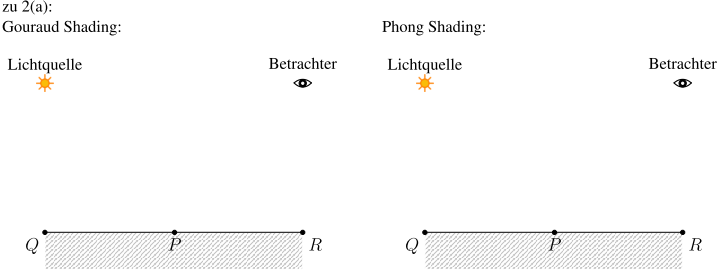
\includegraphics[scale=0.6]{23.png}
\end{center}

\noindent\textbf{PVL 9 - Antwort}

\indent\textbf{1.}

\indent\indent\textbf{(a)}
$I_D = k_d \cdot l_d \cdot max(<n, \ell  >,0)$

\begin{equation}
    \begin{split}
            I_A & = k_d \cdot l_d \cdot max(<n_A,\ell _A>,0)\\
    &= \begin{pmatrix}\frac{1}{2} \\ 1 \\ 1 \end{pmatrix} \cdot \begin{pmatrix} 1 \\ 0 \\ \frac{1}{2} \end{pmatrix} \cdot max(<\begin{pmatrix} -1 \\ 0 \\ 0 \end{pmatrix},\frac{1}{3}\cdot \begin{pmatrix} 2\\ 2 \\ -1 \end{pmatrix}>,0) \\
        &=0
    \end{split}
\end{equation}

\qquad $I_B = k_d\cdot l_d\cdot max(<n_B,\ell _B>,0) = \frac{2}{3}$

\qquad $I_C = k_d\cdot l_d\cdot max(<n_C,\ell _C>,0) = \frac{2}{3}$

\qquad $I_D = 0\alpha  + \frac{2}{3}\beta + \frac{2}{3}\gamma,\ \alpha + \beta+\gamma = 1,\ \alpha ,\ \beta,\ \gamma \geq 0$

\indent\indent\textbf{(b)}
$n = \alpha\begin{pmatrix}-1\\0\\0 \end{pmatrix} + \beta\begin{pmatrix}0\\1\\0 \end{pmatrix} + \gamma \begin{pmatrix}0\\0\\-1 \end{pmatrix}=\begin{pmatrix}-\alpha\\\beta\\-\gamma \end{pmatrix}$ 

\qquad $\ell = norminiert(P_l - (\alpha A+\beta B + \gamma C))$
\\
\\
\indent\textbf{2.}

\indent\indent\textbf{(a)}

\begin{figure}[htb]
    \centering
    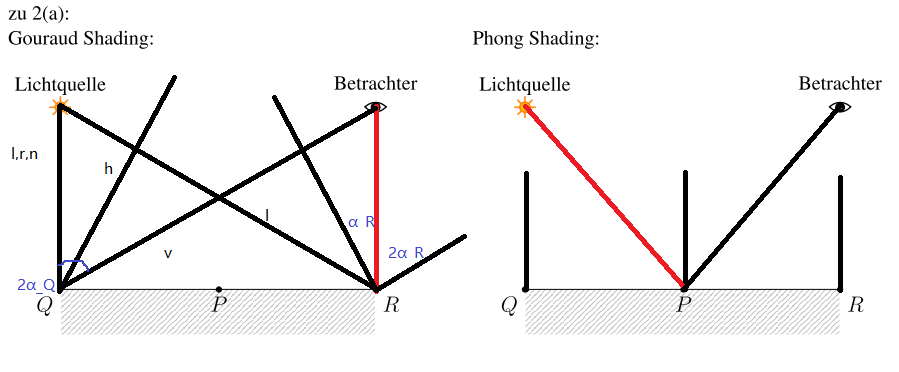
\includegraphics[width=0.7\textwidth]{123.png}
\end{figure}

\indent\indent\textbf{(b)}

\begin{center}

$l_Q=k_s \cdot l_s \cdot <n_Q,h_Q>^s$

$h_Q = \frac{v+\ell}{|v+\ell|} = \frac{1}{\sqrt{7}}\begin{pmatrix}\sqrt{3}\\2\\0\end{pmatrix}$

$\Rightarrow l_Q=\frac{768}{2401}$

$l_R=k_s\cdot l_s \cdot<n_R, h_R>^s$

$h_R=\frac{v+\ell}{|v+\ell|} = \frac{1}{\sqrt{7}}\begin{pmatrix}-\sqrt{3}\\2\\0\end{pmatrix}$

$\Rightarrow l_Q=\frac{768}{2401}$   

$\Rightarrow I_P=\frac{1}{2}\cdot l_Q + \frac{1}{2}\cdot l_R = \frac{768}{2401}$

\end{center}















































\end{document}